%% Copernicus Publications Manuscript Preparation Template for LaTeX Submissions
%% ---------------------------------
%% This template should be used for copernicus.cls
%% The class file and some style files are bundled in the Copernicus Latex Package, which can be downloaded from the different journal webpages.
%% For further assistance please contact Copernicus Publications at: production@copernicus.org
%% https://publications.copernicus.org/for_authors/manuscript_preparation.html


%% Please use the following documentclass and journal abbreviations for preprints and final revised papers.

%% 2-column papers and preprints
\documentclass[journal abbreviation, manuscript]{copernicus}


%% Journal abbreviations (please use the same for preprints and final revised papers)


% Advances in Geosciences (adgeo)
% Advances in Radio Science (ars)
% Advances in Science and Research (asr)
% Advances in Statistical Climatology, Meteorology and Oceanography (ascmo)
% Aerosol Research (ar)
% Annales Geophysicae (angeo)
% Archives Animal Breeding (aab)
% Atmospheric Chemistry and Physics (acp)
% Atmospheric Measurement Techniques (amt)
% Biogeosciences (bg)
% Climate of the Past (cp)
% DEUQUA Special Publications (deuquasp)
% Earth Surface Dynamics (esurf)
% Earth System Dynamics (esd)
% Earth System Science Data (essd)
% E&G Quaternary Science Journal (egqsj)
% EGUsphere (egusphere) | This is only for EGUsphere preprints submitted without relation to an EGU journal.
% European Journal of Mineralogy (ejm)
% Fossil Record (fr)
% Geochronology (gchron)
% Geographica Helvetica (gh)
% Geoscience Communication (gc)
% Geoscientific Instrumentation, Methods and Data Systems (gi)
% Geoscientific Model Development (gmd)
% History of Geo- and Space Sciences (hgss)
% Hydrology and Earth System Sciences (hess)
% Journal of Bone and Joint Infection (jbji)
% Journal of Micropalaeontology (jm)
% Journal of Sensors and Sensor Systems (jsss)
% Magnetic Resonance (mr)
% Mechanical Sciences (ms)
% Natural Hazards and Earth System Sciences (nhess)
% Nonlinear Processes in Geophysics (npg)
% Ocean Science (os)
% Polarforschung - Journal of the German Society for Polar Research (polf)
% Primate Biology (pb)
% Proceedings of the International Association of Hydrological Sciences (piahs)
% Safety of Nuclear Waste Disposal (sand)
% Scientific Drilling (sd)
% SOIL (soil)
% Solid Earth (se)
% State of the Planet (sp)
% The Cryosphere (tc)
% Weather and Climate Dynamics (wcd)
% Web Ecology (we)
% Wind Energy Science (wes)

%% \usepackage commands included in the copernicus.cls:
%\usepackage[german, english]{babel}
%\usepackage{tabularx}
%\usepackage{cancel}
%\usepackage{multirow}
%\usepackage{supertabular}
%\usepackage{algorithmic}
%\usepackage{algorithm}
%\usepackage{amsthm}
%\usepackage{float}
%\usepackage{subfig}
%\usepackage{rotating}
%\usepackage{geometry}
%\usepackage{booktabs}
%\usepackage{siunitx}
\usepackage{graphicx}
\usepackage{rotating}
\usepackage{longtable}
\usepackage{booktabs}
\usepackage[version=4]{mhchem}
\begin{document}

\title{GLOBAL PREDICTION OF TOTAL ORGANIC CARBON IN MARINE SEDIMENTS USING DEEP NEURAL NETWORKS}

\Author[1,2]{Naveenkumar}{Parameswaran}
\Author[1]{Everardo}{Gonz\'{a}lez}
\Author[3]{Ewa}{Burwicz-Galerne}
\Author[2]{Malte}{Braack}
\Author[1]{Klaus}{Wallmann}



\affil[1]{GEOMAR Helmholtz Centre for Ocean Research Kiel}
\affil[2]{University of Kiel}
\affil[3]{MARUM - Center for Marine Environmental Sciences, University of Bremen}


%% If authors contributed equally, please mark the respective author names with an asterisk, e.g. "\Author[2,*]{Anton}{Smith}" and "\Author[3,*]{Bradley}{Miller}" and add a further affiliation: "\affil[*]{These authors contributed equally to this work.}".


\correspondence{NAVEENKUMAR PARAMESWARAN (nparameswaran@geomar.de)}

\runningtitle{TEXT}

\runningauthor{TEXT}





\received{}
\pubdiscuss{} %% only important for two-stage journals
\revised{}
\accepted{}
\published{}

%% These dates will be inserted by Copernicus Publications during the typesetting process.


\firstpage{1}

\maketitle



\begin{abstract}
Spatial predictions of total organic carbon (TOC) concentrations and stocks are crucial for understanding marine sediments' role as a significant carbon sink in the global carbon cycle. In this study, we present a geospatial prediction of TOC concentrations and stocks at a 5 x 5 arc minute grid scale, using a deep learning model — a novel machine learning approach based on a new compilation of over 22,000 global TOC measurements and a new set of predictors, such as seafloor lithologies, grain size distribution, and an alpha-chlorophyll satellite data. In our study, we compared the predictions and discuss the limitations from various machine learning methods. Our findings reveal that the neural network approach outperforms methods such as k Nearest Neighbors and random forests, which tend to overfit to the training data, especially in highly heterogeneous and complex geological settings. We provide estimates of mean TOC concentrations and total carbon stock in both continental shelves and deep sea settings across various marine regions and oceans. Our model suggests that the upper 10 $cm$ of oceanic sediments harbors approximately 171 $Pg$ of TOC stock and has a mean TOC concentration of 0.68\%. Furthermore, we introduce a standardized methodology for quantifying predictive uncertainty using Monte Carlo dropout and present a map of information gain, that measures the expected increase in model knowledge achieved through in-situ sampling at specific locations which is pivotal for sampling strategy planning.
\end{abstract}




\introduction  
\label{sec:Introduction}



Burial of particulate organic carbon in marine sediments removes carbon dioxide (\ce{CO2}) from the atmosphere and generates molecular oxygen (\ce{O2}) that accumulates in the atmosphere \citep{Berner1982, HEDGES199581}. It is a key process in the global carbon cycle that largely controls the atmospheric partial pressures of \ce{O2} and \ce{CO2} on geological timescales \citep{Berner1982, bernerbook2004}. The mechanisms controlling concentrations, standing stocks, degradation and accumulation rates of organic carbon at the seabed are, however, complex and remain a topic of active research \citep{ARNDT201353, burdige2007, HEDGES199581, larowe2020a, Bradley2022}.  Furthermore, present estimates on the spatial distribution of sedimentary carbon concentrations and stocks across the global ocean, including shelf regions, are limited due to sparse data and the large spatial variability observed in shelf deposits \citep{atwood2020, diesing2021, LeeTOCkNN, legge2020, SEITER20042001}. Against this background, an improved map of global organic carbon concentrations and stocks in marine surface sediments, including the continental shelf, could help to better understand processes governing the turnover and accumulation of organic carbon at the seabed.


Shelf and deep-sea regions are separate environments. Surface sediments deposited on the continental shelf are mostly composed of clay, silt, and sand delivered by rivers and continental erosion, while pelagic sediments deposited at the deep-sea floor contain large amounts of biogenic material (carbonate, biogenic opal) produced by marine plankton \citep{bernerAndBerner2012}. Moreover, shelf deposits are frequently eroded, reworked and redistributed by bottom currents and intensively mixed and irrigated by benthic biota \citep{ALLER1998143, boudreau1997diagenetic, song2022global}. Shelf sediments are also affected by human activities such as bottom-trawling and dredging that erode and disperse large sediment volumes \citep{Sala2021}. Organic carbon within shelf and deep-sea deposits constitutes only a minor fraction of the sediment mass. It is composed of of both reactive and inert organic matter where the reactive fraction is subject to fast biological degradation processes \citep{Hiddink2023}. Degradation rates increase with temperature and oxygen exposure \citep{ARNDT201353, HEDGES199581}. Global warming and resuspension of anoxic shelf sediments in oxygen-bearing bottom waters by e.g. bottom-trawling, therefore, enhance organic carbon degradation and induce significant \ce{CO2} emissions at the seabed that may contribute to global climate change \citep{Hiddink2023, Sala2021}. An improved understanding of carbon stocks in surface sediments and their spatial distribution is, hence, also needed to better constrain present and future \ce{CO2} fluxes at the shelf seabed \citep{atwood2020}.


Sedimentary organic carbon concentrations are typically reported as total organic carbon (TOC in weight percent), which includes particulate organic carbon bound to sediment grains and a minor contribution by organic carbon dissolved in sediment porewater \citep{HEDGES199581}. TOC varies between different geological environments \citep{Emerson1988}. Fine-grained shelf and delta sediments deposited close to river mouths typically contain 0.5 – 1.0\% TOC at 0 – 10 $cm$ sediment depth \citep{Berner1982}. A major fraction of TOC deposited in these environments (up to 67\%) is not formed by marine plankton but produced by land plants \citep{Burdige2005}. Shelf regions where neritic carbonates are formed by corals and other organisms at the seabed contain about 1\% TOC \citep{Berner1982}. However, large parts of the continent shelf (about 50 - 70\%) do not receive sediment inputs and are covered by relict sands \citep{emery1968relict, Hall2002} that contain only minor amounts of TOC (about 0.1\%). Typical deep-sea sediments, that are not associated with high productivity regions, contain about 0.2 – 0.4\% TOC \citep{Baturin2007, Berner1982, LeeTOCkNN, SEITER20042001}. In oceanic upwelling regions with high productivity, large amounts of TOC are rapidly deposited at the seabed such that sedimentary TOC concentrations are usually larger than 1\% and may reach up to 10\% \citep{Berner1982, LeeTOCkNN, SEITER20042001}. Elevated TOC values are also reported for surface sediments deposited in the Arctic Ocean (1.0\%) and the deep basins of the Black Sea (2.0\%) \citep{Berner1982, LeeTOCkNN, SEITER20042001}. Considering these observations, the global mean TOC concentration in both shelf and deep-sea sediments seems to be close to 0.5 to 1.0\%.


The inventory or standing stock of TOC in surface sediments (in mass of carbon per seafloor area) is calculated by multiplying TOC concentrations with the dry bulk density of sediments and the thickness of the considered surface layer. Different methods have been applied to derive the standing stock of TOC at regional and global scales. An early estimate based on limited data and expert knowledge concluded that the global TOC inventory is 146 $Pg$ TOC for a 30 $cm$ thick surface layer \citep{Emerson1988}. The first estimate of the global TOC inventory derived by a machine-learning approach (k-Nearest Neighbors (kNNs)) using an extended database (5,623 data points) yielded a global inventory of 87 $\pm$ 43 $Pg$ TOC in the top 5 $cm$ layer \citep{LeeTOCkNN}. In subsequent publications with an extended database (11,574 sediment cores) and a more advanced machine-learning approach (random forest model), the global inventory was estimated as 2322 $Pg$ TOC for the top 1 $m$ of the sediment column \citep{atwood2020}. This inventory exceeds the global TOC inventory in terrestrial soils and suggests that TOC in marine surface sediments is the largest TOC pool at the surface of the Earth \citep{atwood2020}. Another estimate of the global TOC inventory was derived by reactive transport modeling of sedimentary processes employing a range of global datasets \citep{larowe2020b}. This model yields a global inventory of 171 $Pg$ TOC for the top 10 $cm$ affected by biological mixing processes.


Since about 70\% of the Earth's surface is covered by oceans, and sampling sediments at the seafloor is costly, data coverage will always be sparse. Therefore, advanced methods are required to derive spatial information on sediment properties from a limited number of point measurements. Machine learning approaches, which have rapidly advanced in recent years, are the most promising approach to tackle this challenge. So far, k-nearest neighbors and random forest models have been applied to derive global maps of sediment porosity \citep{Martin2005Porosity}, TOC concentration \citep{LeeTOCkNN}, TOC inventory \citep{atwood2020}, sedimentation rate \citep{restrepo2, Restreppo2020}, and regional estimates of TOC accumulation rates \citep{diesing2021}. However, machine-learning techniques have their own challenges and limitations. Overfitting issues are often encountered, and a standardized approach for estimating predictive uncertainty has not yet been established \citep{LeeTOCkNN}.



Against this background, this paper aims to derive more robust and better-resolved maps of TOC concentrations and inventories for the global ocean, including the continental shelf, based on a new larger TOC measurement database and an extended collection of predictors to improve the accuracy at highly heterogeneous and undersampled geological settings. We compiled an enlarged database of TOC concentrations in surface sediments with 22,192 entries and applied a deep neural network (DNN) as a more advanced machine-learning approach. The global ocean was divided into two different domains (shelf and deep-sea), and the network was trained separately for each of these domains. Moreover, we developed new methods to quantify predictive uncertainties and information gain.



\section{Materials}
\subsection{Features}
\label{sec:features}
An extensive repository of features from both the sea surface and the seafloor at a 5 x 5 arc minute grid resolution has been compiled. It is based on features reported in \cite{LeeTOCkNN, restrepo2, HartDavis2021EOT20} and includes a range of oceanographic, geological, geographic, biological, and biogeochemical parameters. Features deemed irrelevant to TOC distributions (e.g. crustal and mantle properties; distance to plate boundary, continental ridges, trenches; seasonal means of sea conductivity, sea oxygen, sea oxygen saturation percentage, sea oxygen utilization, sea temperature) were excluded.


We adopted the spatial mean calculation as the sole averaging method, with a spatial average over a 50 km radius to incorporate neighborhood information alongside raw features. Additional features believed to influence TOC distributions, including total oxygen uptake (respiration rates) at the seabed \cite{TOU_JORGENSEN2022}, sediment characteristics (awaiting citation confirmation), tidal velocities \cite{HartDavis2021EOT20}, and chlorophyll-alpha concentrations at the sea surface \cite{nasaaqua}, were incorporated.



Together, 99 raw feature grids are compiled for a comprehensive representation of the marine environment, providing the necessary input for the neural network analysis in this study to predict total organic carbon content. Most of the depicted features are easily measurable from the sea surface by e.g. satellite observations, making them a reliable dataset compared to the less accessible properties of the seafloor. Feature grids that lack global coverage or are only available at inappropriate resolutions have been resampled, cell centered, and interpolated as needed using various techniques, including machine learning. Overall, a total of 139 features are used in the model, including the spatial averages, that are listed in the supplementary information.



\subsection{TOC Data}
\label{subsec: labels}
The dataset for TOC concentrations (in weight percent) utilized in this study has been compiled from multiple sources. It includes global data sets from \cite{SEITER20042001, romankevich2009organic, mosaic} and regional data sets for the the northern Gulf of Mexico \citep{beazley2003significance} and the North Sea (personal communication, W. Zhang, HEREON). Each label represents a known measurement (TOC concentration) and is paired with the nearest grid point on the 139-feature grids via L2 distance computation, resulting in the association of a feature vector with each label. The labeled data is preprocessed to enhance the reliability and robustness of the dataset for subsequent model development and validation. Coastal regions often exhibit  clustered measurements, potentially resulting in shared feature vectors, as all the measurements lie in the same feature grid cell. To mitigate this, a variance assessment is conducted. Labels associated with feature vectors exhibiting high variance (the standard deviation of the labels is higher than 20\% of the maximum of the labels)  are excluded, while those with low variance are averaged, and the shared feature array is assigned. Also, some data points situated in close proximity to land may have feature values affected by NaN (Not-a-Number, used for undefined numbers) values due to the coarseness of the dataset. To address this, reasonable values are assigned by interpolating from the nearest points, ensuring the overall quality of the dataset. Our database includes a total of 110149 data points (including duplicates from overlap of different sources) that have been consolidated as discussed above such that the TOC database employed in the model is composed of 22192 entries (Figure \ref{fig:toclabels}\footnote{The color maps used for the figures in this paper are from \cite{fabiocramericolormap} and \cite{cmoceancolormap}.}). Both the datasets for labels and features can be downloaded at https://doi.org/10.5281/zenodo.11186224.

\begin{figure}[!htb]
    \includegraphics[width=12cm]{figures/f01.png}
    \caption{Quantitative total organic measurements (i.e., labels) acquired from various sources \citep{SEITER20042001, romankevich2009organic, mosaic, beazley2003significance}. Notably, data point clusters are observed in close proximity to coastal regions.}
    \label{fig:toclabels}
\end{figure}




\section{Methods}
\label{sec:methods}

The primary objective of this study is to build a supervised prediction model that uses feature grid maps as inputs to predict TOC concentrations as outputs. Additionally, we aim to quantify prediction uncertainties using Monte Carlo dropout and information theory techniques. The supervised model is trained using the set of labels (TOC data) and their corresponding feature vectors. Due to the complex patterns in the data, we choose deep learning models, which are good at understanding such patterns.


\subsection{Deep learning model}
Deep Neural Networks (DNNs) have achieved state of the art results on a variety of tasks in ocean observation, prediction, and forecasting of ocean phenomena \citep{reviewAIinMarineScience}. DNN architectures, that are intrinsically non-parametric and non linear, are less susceptible to the curse of dimensionality. They capture complex relationships between features at different levels of abstraction through their hierarchical nature which makes them well-suited to resolve highly complex geoscientific problems \citep{LeCun2015}. 

Here, we propose a multi-layer perceptron (MLP), feed forward DNN to predict global TOC in sediments and an approach to map uncertainty in predictions that serves as a quantifiable measure of information gain from sampling. In contrast to a one-model approach for both deep sea and continental shelves as in previous works \citep{Restreppo2020, restrepo2, Martin2005Porosity, LeeTOCkNN}, separate models are trained and inferred on data from two marine regions: the deep sea (> 200$m$ depth) and the continental shelves (< 200$m$ depth), because of the different parameters that drive the sedimentation process in these regions. The DNN, initialized using the technique proposed by \cite{he2015delving} (initializes parameters of the DNN taking into account the non-linearity of activation functions), consists of 10 layers with 128 nodes each. Batch normalization (which normalizes the inputs of each layer for faster and more stable training) and dropout (which assigns a probability of being deactivated to each node during training and thus prevents overfitting) are applied to each layer for regularization. ReLU (Rectified Linear Unit, a piecewise linear function that outputs 0 for negative inputs and the input itself for positive inputs, introducing non-linearity in the DNN) is used as the activation function.



The Monte Carlo Dropout method is implemented here to estimate uncertainty in the DNN model, leveraging dropout layers as approximate Bayesian inference \citep{MCDropout}. It gives us an ensemble of predictions from different subsets of neurons in the same DNN model. Kullback Leibler (KL) divergence is used to map information gain from the quantified predictive uncertainty. In the field of information theory, KL divergence represents the information gain and is defined as the difference of the cross entropy between the observation and the prediction of an event, and the entropy in the observation of the event \citep{kullbackleibler1951}. In our context, the predicted distribution arises from Monte Carlo dropout prediction ensemble, while the reconstructed observed distribution is modeled with a normal distribution with the predicted value as a mean and the standard deviation of 0.05 TOC\%, arising from both technical handling and the precision of the weighing tool \citep{pape2020}. The mathematical formulation of the entropy and the cross entropy is detailed in the supplement.

In other words, information gain measures the expected increase in model knowledge achieved through in-situ sampling at a specific location. This concept provides a strategic guide for determining optimal sampling strategies to refine our model's representation of the real world.

%


\section{Results and Discussions}
Understanding the global distribution of TOC concentrations and stocks is crucial for advancing our knowledge of the carbon cycle and sedimentary environments worldwide. Before delving into the prediction maps from the DNN, we first compare the performance of three methods: DNNs, kNNs, and random forests. Separate models are run for deep-sea and continental shelf regions, and the outcomes are summarized in Table \ref{tab:kNNRF}. For kNN, 5 neighbors were utilized for continental shelves, and 4 for the deep sea, based on a sensitivity analysis with respect to model performance. Random forests employed 100 estimators for both marine regions. This comparison sets the groundwork for a detailed exploration of DNN results, offering insights into its effectiveness compared to other established methods. Notably, random forest and kNN algorithms exhibit higher correlation coefficients and superior overall performance on the training dataset than the DNN, however, the DNN outperforms both the other algorithms in the test data performance. This discrepancy suggests a potential overfitting issue, where the kNN and random forest models may have become specialized in learning the training data. Nonetheless, they are useful learning algorithms when computational resources are constrained. More detailed analysis of the results of kNN and random forests are provided in the supplementary information. The correlation plot between measured and predicted data shows similar errors for the training and test data sets which confirms that the DNN-model largely avoids overfitting (Figure \ref{fig:correlationPlot}).

\begin{table}[h]
  \centering
  \begin{tabular}{|l|c|c|c|c|}
    \hline
    \textbf{Method} & \multicolumn{2}{c|}{\textbf{Train data}} & \multicolumn{2}{c|}{\textbf{Test data(15\% of all data)}} \\
    \hline
           & \textbf{Pearson CC} & \textbf{R-squared} & \textbf{Pearson CC} & \textbf{R-squared} \\
    \hline
    \textbf{kNN} & 0.927 & 0.859 & 0.8435 & 0.6747 \\
    \hline
    \textbf{Random forests} & \textbf{0.986} & \textbf{ 0.969} & 0.8470 & 0.6949 \\
    \hline
    \textbf{DNN} & 0.909 & 0.807 & \textbf{0.853} & \textbf{0.725} \\
    \hline
  \end{tabular}
    \caption{Comparison of machine learning methods based on performance metrics: Pearson correlation coefficient (Pearson CC) and coefficient of determination (R-Squared) for the training and testing data. The train:test data ratio is 85:15.}
  \label{tab:kNNRF}
\end{table}





\begin{figure}
    \centering
    \includegraphics[width = 4.3 cm]{figures/f02.png}
    \caption{Correlation plot between measured (labels) and predicted data (targets) using DNN, with particular emphasis on the test dataset (purple points) to assess the model's generalization performance. The minimal difference observed between train and test errors serves as an indicator of the model's ability to avoid overfitting.}
    \label{fig:correlationPlot}
\end{figure}



\begin{figure}
        \centering
        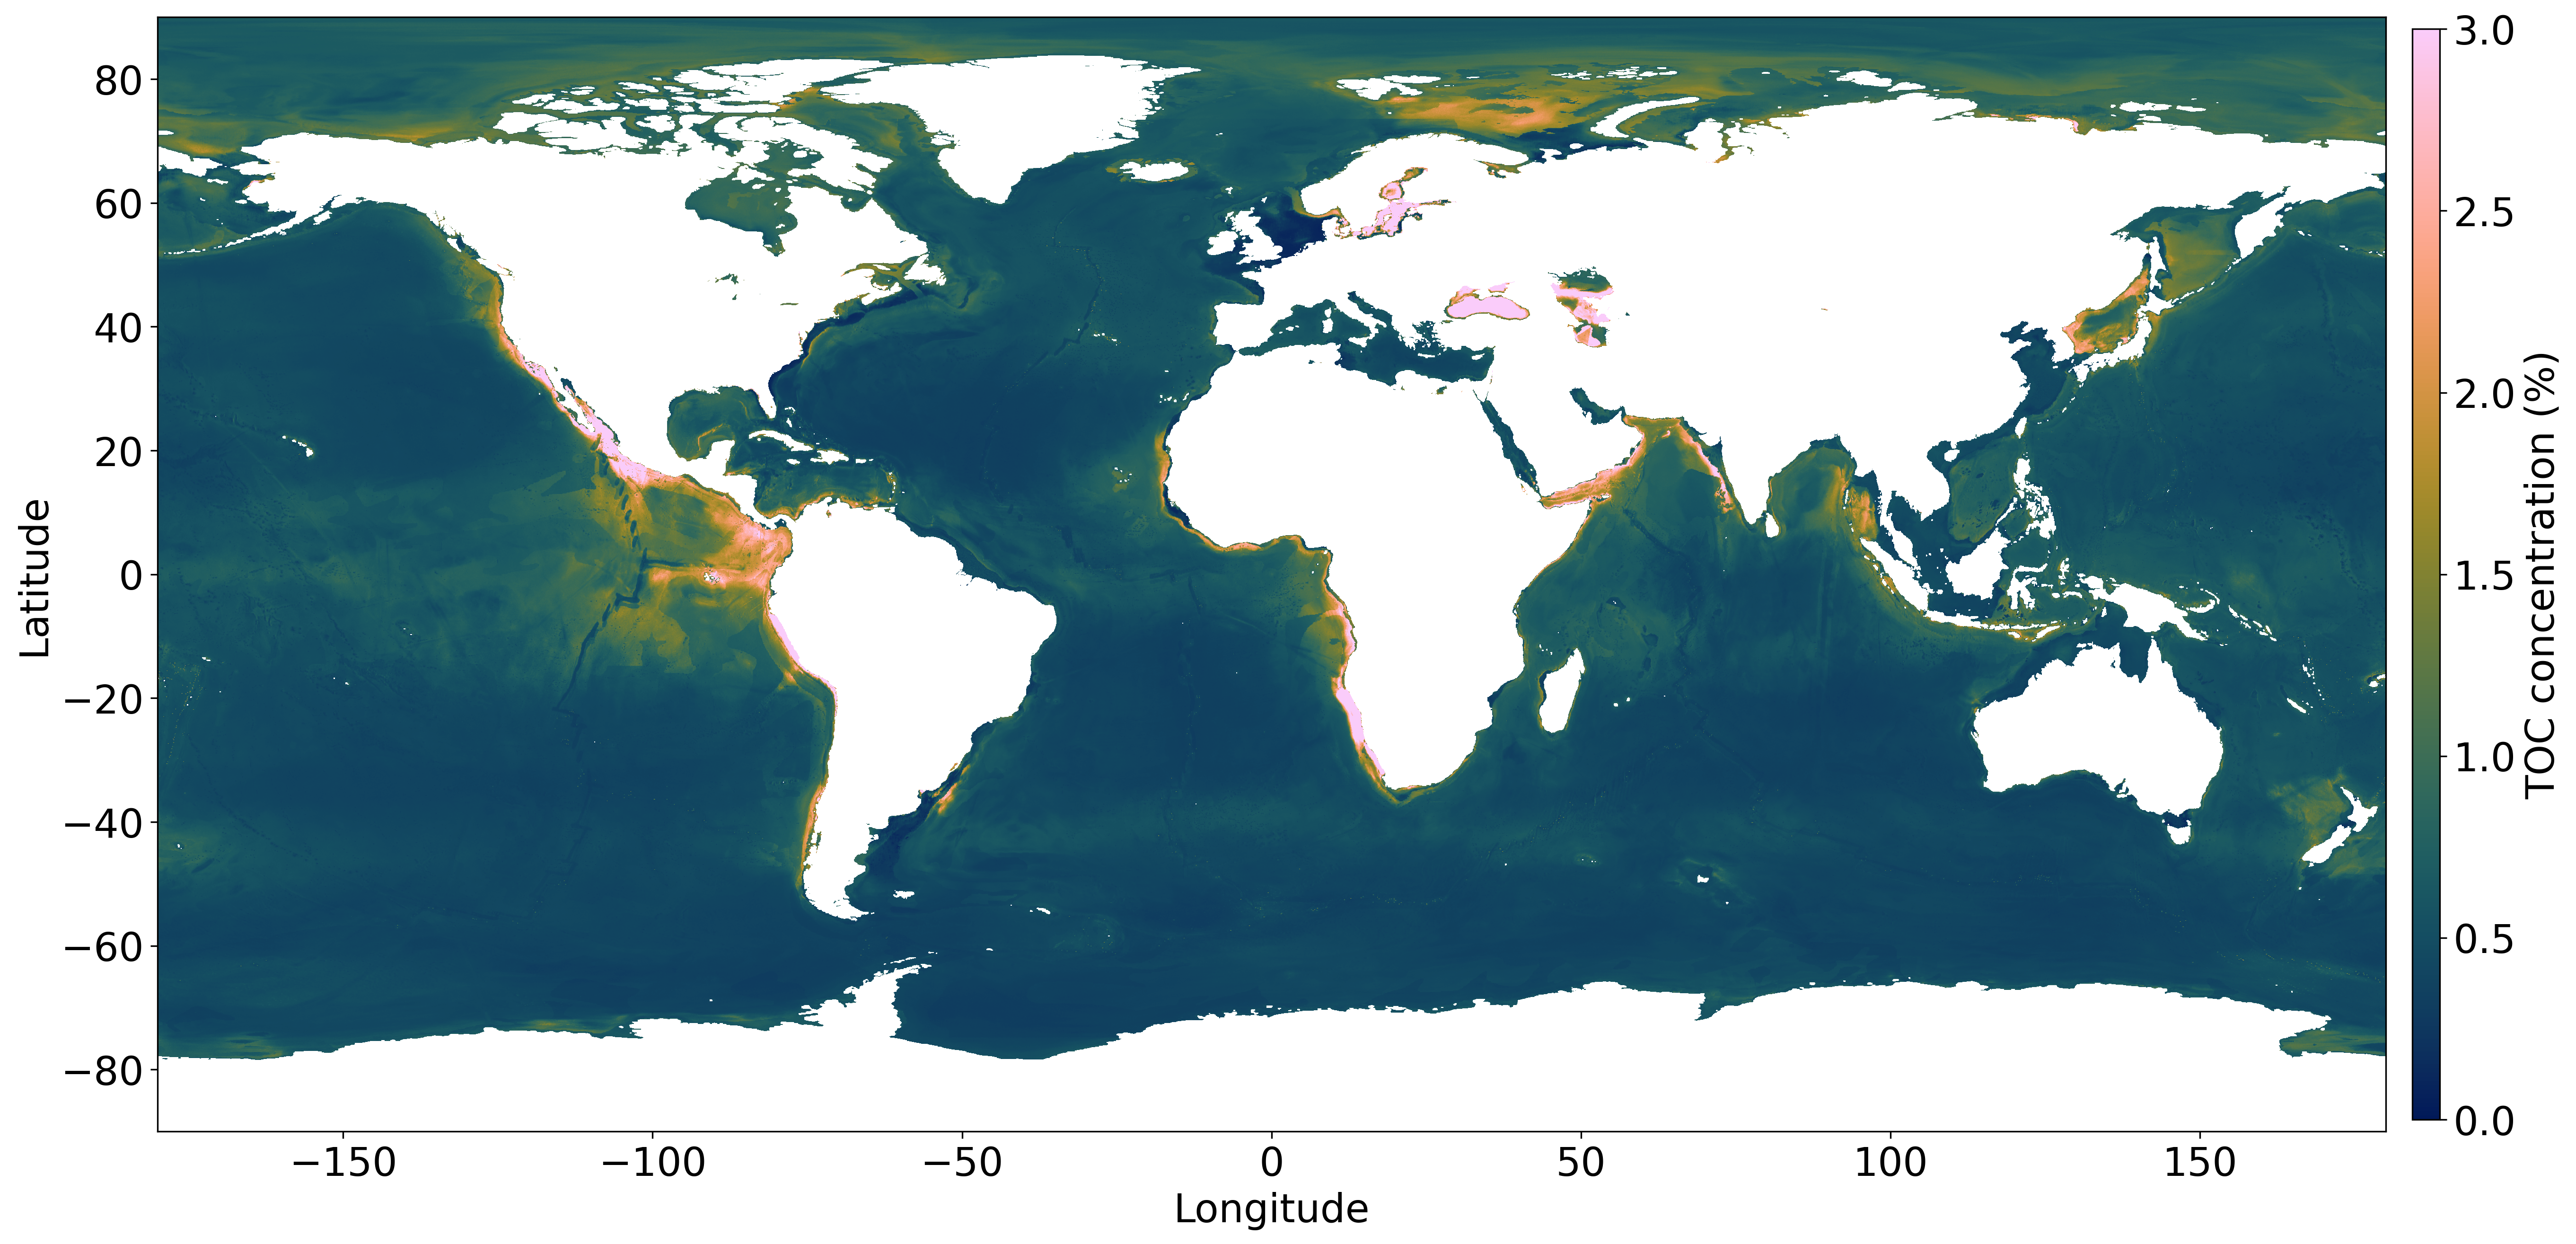
\includegraphics[width = 12cm]{figures/f03.png}
        \caption{Global prediction map of the TOC concentration using a DNN.}
        \label{fig:tocPercent}
\end{figure}



Our DNN-based map of TOC concentrations (Figure \ref{fig:tocPercent}) shows similarities to maps previously published by \cite{SEITER20042001} and \cite{LeeTOCkNN}, who used geostatistical methods and a kNN model, respectively. All maps show elevated concentrations in the Arctic region and in upwelling areas located along the western continental margins of America and Africa, the equatorial Pacific, and the Arabian Sea. This pattern can be explained by elevated rates of marine primary and export production in upwelling regions delivering large fluxes of TOC to the seabed. The low TOC values in the open oceans are related to lower productivity and the large water depths limiting the TOC flux to the deep-sea floor. The predictions in Figure \ref{fig:tocPercent} are also consistent with the early work on TOC distributions by \cite{Berner1982} and \cite{Emerson1988}, showing low TOC values in the open oceans and elevated values for upwelling regions and the Arctic region. The high TOC concentrations predicted for the Black Sea and Baltic Sea (Figure \ref{fig:tocPercent}) are probably related to the lack of oxygen in bottom waters of these marginal seas that promotes TOC preservation \citep{HEDGES199581}. The map published by \cite{LeeTOCkNN} shows several large areas in the open Pacific that have unusually high TOC concentrations. These patches are probably not realistic since they do not appear in other maps and are not consistent with our understanding of the TOC cycle. They may be artifacts generated by the kNN method and the sparse data coverage in these regions. Our new map avoids these artifacts and offers much better coverage and spatial resolution for the shelf region than previous maps \citep{SEITER20042001}. This feature and the avoidance of overfitting are the major advances achieved by our modeling approach.


\begin{figure}
        \centering
        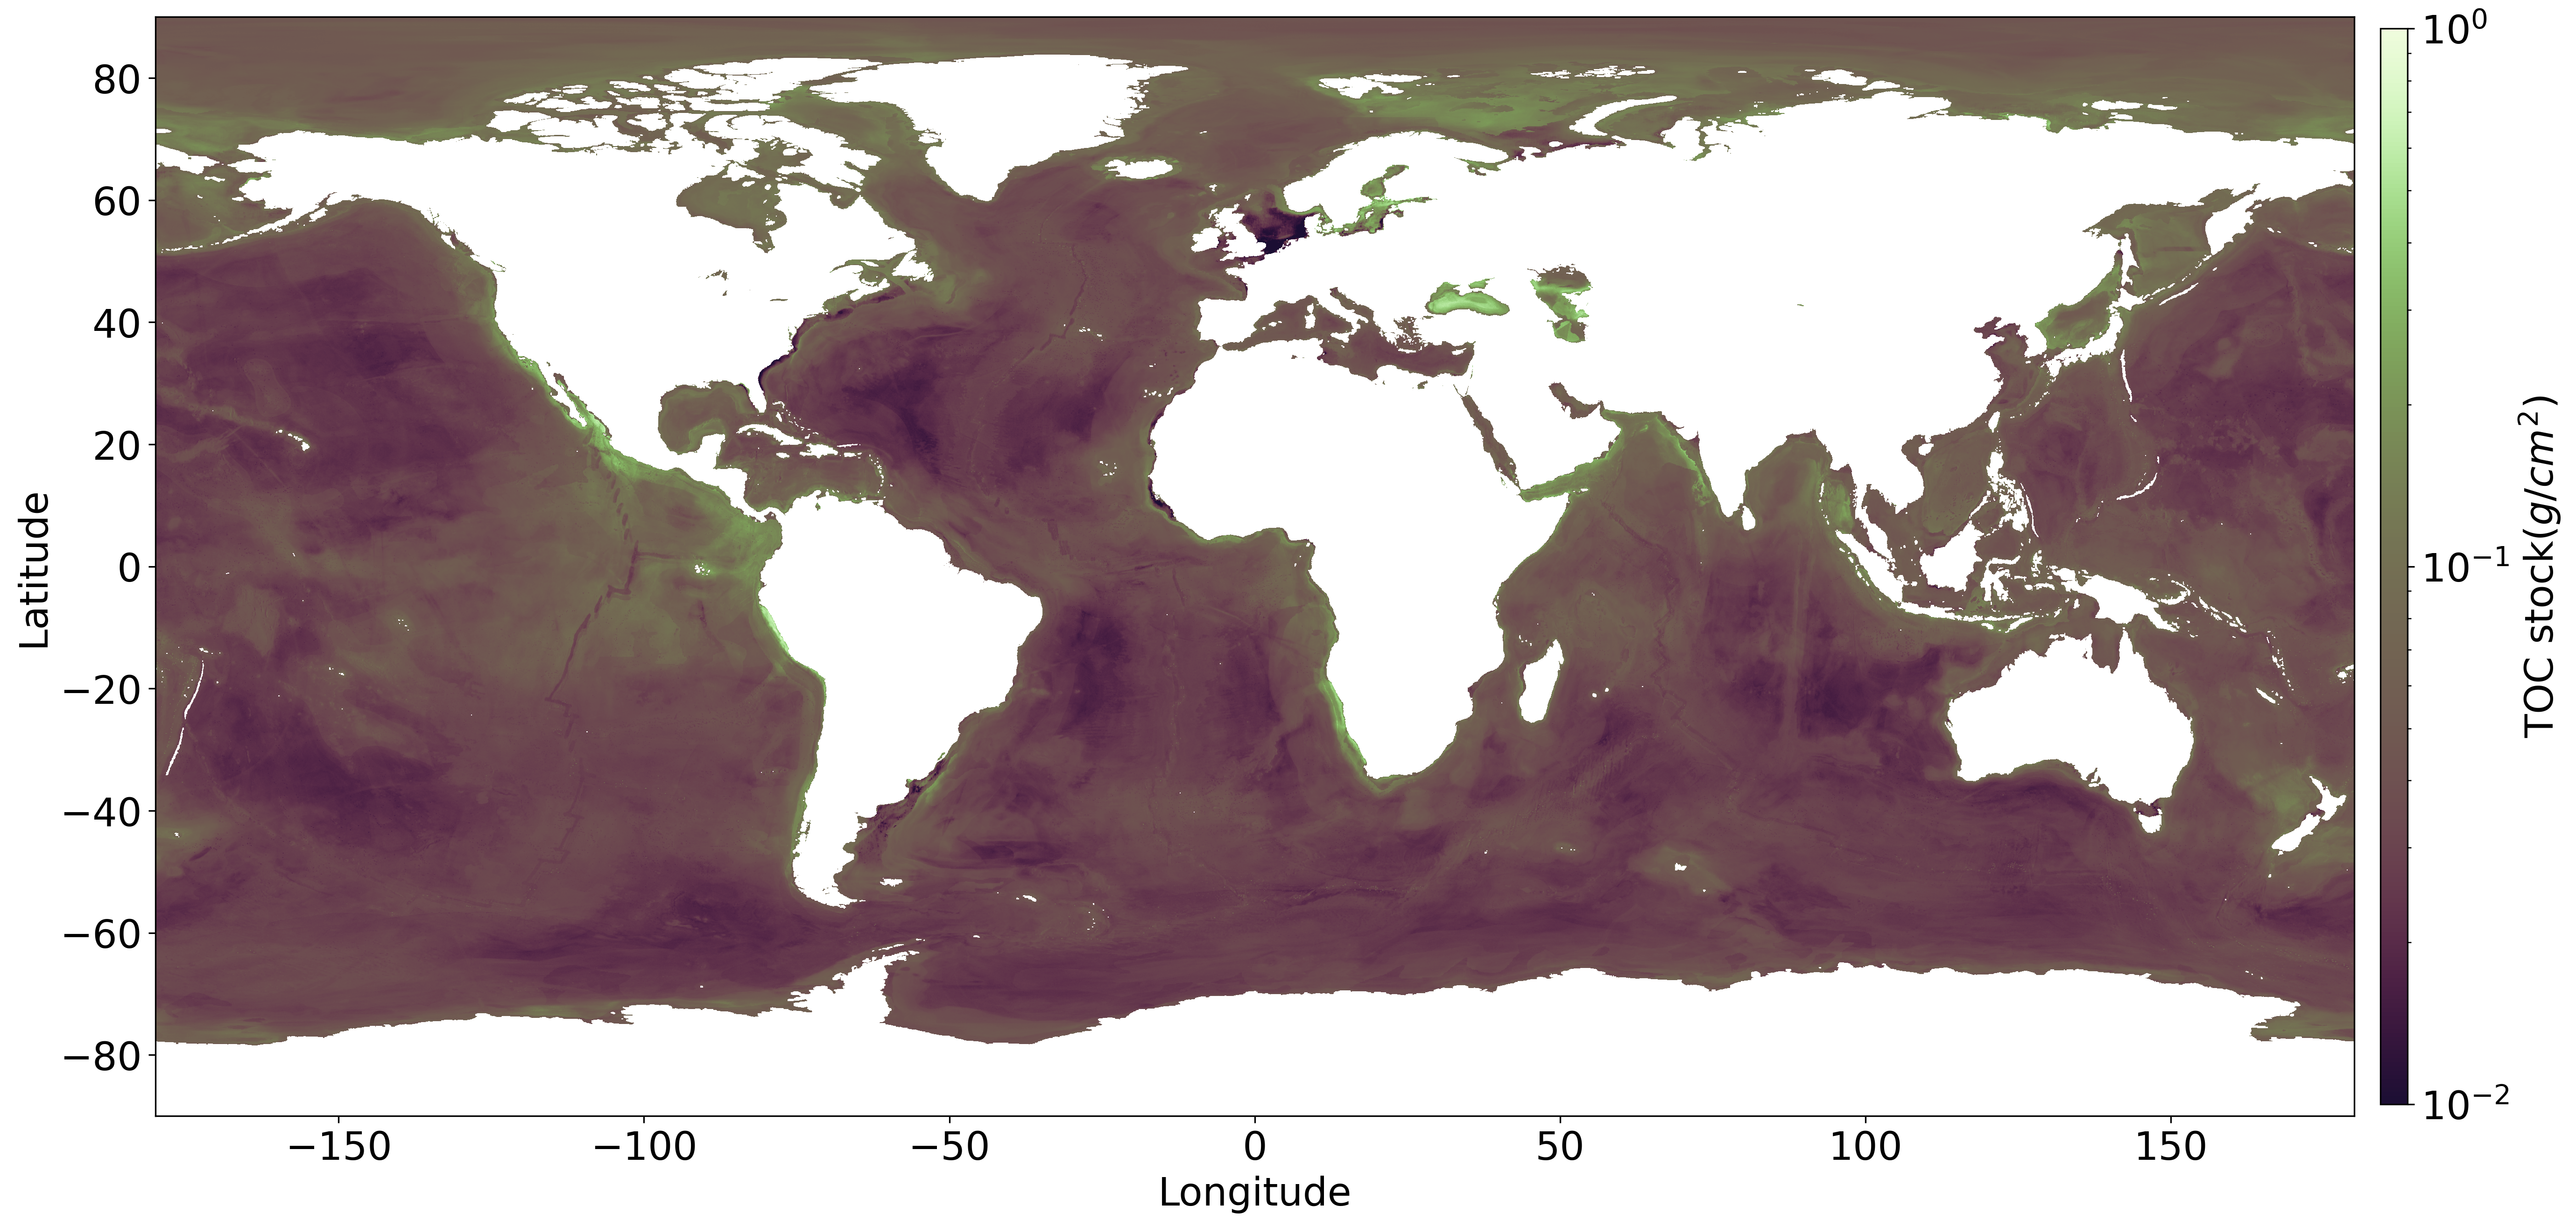
\includegraphics[width = 12cm]{figures/f04.png}
        \caption{TOC stock map.}
        \label{fig:tocStock}
\end{figure}

We also produced a map of TOC stocks for the global ocean (Figure \ref{fig:tocStock}). The TOC stock was calculated using the global porosity grid provided by \cite{Martin2005Porosity} and a density of dry solids ($d_s$) of $2.6 g/cm^3$. We performed the calculation for the top 10 $cm$ of the sediment column since our TOC data have been measured within this thin surface layer. Moreover, the top 10 $cm$ are the most vulnerable and dynamic part of the sedimentary TOC pool since they are subject to frequent biological and physical mixing  processes \citep{song2022global} and are affected by human interventions such as bottom trawling \citep{Sala2021}. The TOC stocks are calculated as:

\begin{equation}
 \text{TOC stock} = (1 - \text{porosity}) \times d_s \times \text{TOC concentration} \times \text{10 cm}   
\end{equation}


\begin{table}[htbp]

\centering
\begin{tabular}{|p{0.2\textwidth}|p{0.1\textwidth}|p{0.1\textwidth}|p{0.1\textwidth}||p{0.1\textwidth}|p{0.1\textwidth}|p{0.1\textwidth}|}
\hline
& \multicolumn{3}{c||}{\textbf{Continental Shelves}} & \multicolumn{3}{c|}{\textbf{Deep Sea}} \\
\hline
\textbf{Region} & \textbf{Sum of TOC stock(\$Pg\$)} & \textbf{Area (million km\textsuperscript{2})} & \textbf{Mean TOC concentration(\%)} & \textbf{Sum of TOC stock(\$Pg\$)} & \textbf{Area (million km\textsuperscript{2})} & \textbf{Mean TOC concentration(\%)} \\
\hline
\hline
Arctic Ocean & 5.24& 5.72 & 0.88 & 6.98 & 9.46 & 0.87 \\
\hline
Indian Ocean & 2.52& 4.06 & 0.59 & 29.82 & 67.10 & 0.64 \\
\hline
Mediterranean Region & 0.60& 0.65 & 0.97 & 2.16 & 2.27 & 1.18 \\
\hline
North Atlantic Ocean & 2.55& 4.26 & 0.57 & 17.07 & 37.46 & 0.66 \\
\hline
North Pacific Ocean & 2.58& 3.83 & 0.63 & 33.76 & 73.42 & 0.73 \\
\hline
South Atlantic Ocean & 1.08& 1.86 & 0.72 & 15.54 & 38.67 & 0.62 \\
\hline
South China and Easter Archipelagic Seas & 1.60& 3.00 & 0.50 & 2.61 & 3.74 & 0.87 \\
\hline
South Pacific Ocean & 1.19& 1.46 & 0.96 & 36.72 & 83.81 & 0.64 \\
\hline
Southern Ocean & 0.20& 0.57 & 0.56 & 7.63 & 20.16 & 0.52 \\
\hline
Baltic Sea$^*$ & 0.84 & 0.39 & 3.36 & & & \\
\hline
Caspian Sea$^*$ & 0.81 & 0.38 & 2.55 & & & \\
\hline
\hline
\textbf{Total} & 19.21 & 26.20 & 0.75 & 152.30 & 336.08 & 0.66 \\
\hline
\end{tabular}
\caption{TOC Stock in the continental shelves and deep sea regions of different marine domains. $^*$The total sums and the mean concentrations in the continental shelves include the Baltic Sea and the Caspian Sea. Without these regions, the total TOC stock in continental shelves is 17.56 $Pg$, area of the continental shelves is 25.42 million km\textsuperscript{2} and the mean TOC concentration is 0.69\%. Visualisation of the TOC stock in the oceans is provided in the supplementary information.}
\label{tab:TOCStockOcean} 
\end{table}









The TOC stock is computed for global oceans and major seas \citep{FlandersMarineInstitute2021}, focusing on both continental shelves and deep-sea regions within each ocean and sea and is shown in Table \ref{tab:TOCStockOcean}. Notably, the mean TOC concentration in continental shelves exhibits significant variability across regions. 

According to our  model, most the TOC stock can be found in the vast deep-sea basins of the Pacific, Indian and Atlantic oceans which is due to the large area of these basins (Table \ref{tab:TOCStockOcean}). The shelf region harbors 11.2\% of the global stock (Table \ref{tab:TOCStockOcean}, including Baltic Sea and Caspian Sea), similar to the fraction, previously derived by \cite{atwood2020} who suggested that 11.5\% of the global TOC stock is located on the continental shelves. The global TOC stock derived from our model amounts to 171.5 $Pg$ carbon for the 10 $cm$ layer consider in our calculations (Table \ref{tab:TOCStockOcean}). This value is close to the global stock in the top 10 $cm$ derived by reactive transport modeling (170 $Pg$, \cite{larowe2020b}). The other stock estimates were calculated applying a range of sediment thicknesses. When normalized to 10 $cm$, the stocks reported by \cite{LeeTOCkNN} amounts to 174 $Pg$ while the stock derived by \cite{atwood2020} results as 232 $Pg$ carbon. The first stock estimate, that was based on expert knowledge and a limited data base, corresponds to only 49 $Pg$ carbon when normalized to 10 $cm$ \citep{Emerson1988} which is lower than our estimate.

According to our DNN-model, the mean TOC concentration in continental shelves sediments, excluding the Baltic Sea and the Caspian Sea (0.69\%) is close to the concentration in deep-sea sediments (0.66\%, Table \ref{tab:TOCStockOcean}). This is a surprising result since the high marine productivity and low water depths on the shelf induce high TOC fluxes to the seabed that should result in elevated TOC concentrations in surface sediments. Moreover, large amounts of terrestrial particulate organic carbon (POC) produced by land plants are deposited in shelf sediments \citep{Burdige2005} which should further increase TOC concentrations on these deposits. However, TOC concentrations in shelf surface sediments are diminished by a number of factors: i.  frequent biological and physical reworking that accelerates TOC degradation processes \citep{song2022global}, ii. dilution of TOC by inorganic material (clay, silt, sand) in delta deposits and other shelf regions with high sedimentation rates \citep{Berner1982}, iii. strong bottom currents that inhibit sediment deposition such that large shelf areas are covered by relict coarse-grained sediments that were deposited in the geological past and do not contain significant amount of TOC \citep{emery1968relict}, iv: frequent bottom trawling that exposes sedimentary TOC to oxygen and accelerates TOC degradation \citep{atwood2020}. According to our DNN-model, these factors decrease TOC concentrations in shelf sediments to such to degree that they attain mean values that are close to those observed in deep-sea sediments (Table \ref{tab:TOCStockOcean}). 
The regions with the highest information gain (Figure \ref{fig:informationgain}) are predominantly situated on continental shelves. Despite the Norwegian Trench exhibiting a high total organic carbon percentage, sufficient measurements in the North Sea contribute to lower uncertainty, resulting in a lower information gain. Notably, the Gulf of Mexico, Carribean sea, North Pacific Ocean and the western coast of Madagascar exhibit higher information gain due to a scarcity of measurement. Clusters of measurements, such as those in the North Sea, East China Sea, or North Atlantic Ocean, show lower information gain. Significantly, our analysis also reveals that an abundance of measurements does not necessarily correspond to lower information gain, and vice versa, as in the case of the south west coast of Africa. Information gain depends not only on the geographical proximity of measurements but also on their proximity in the parameter space and the congruence of the measurements made there. 

\begin{figure}
    \centering
    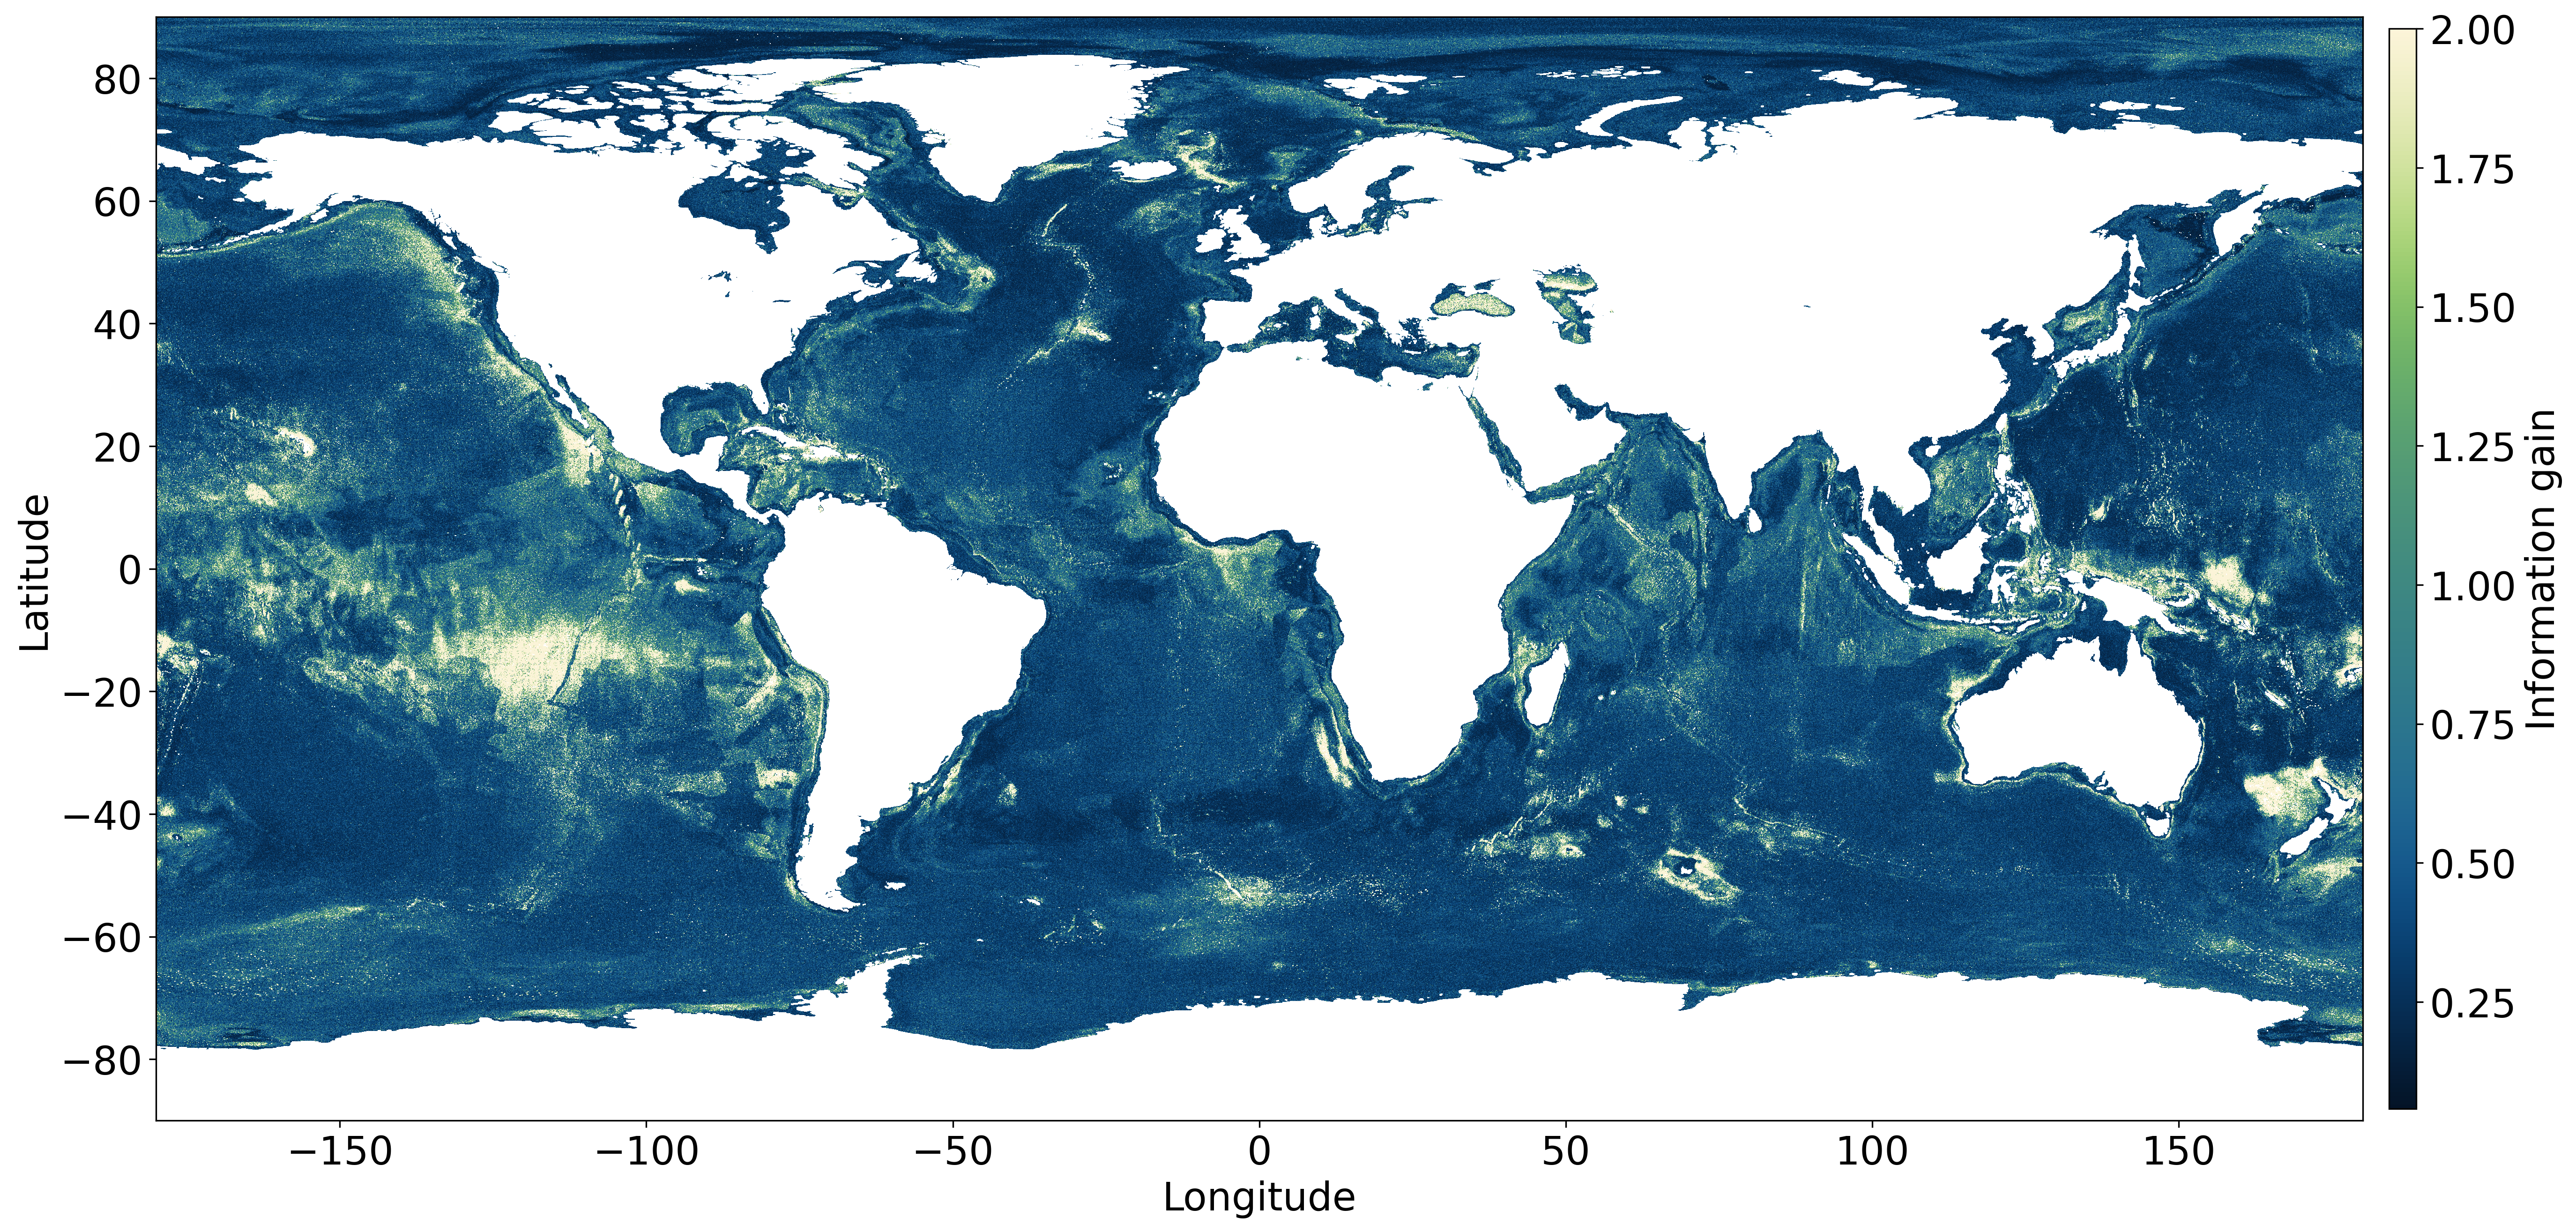
\includegraphics[width = 12cm]{figures/f05.png}
    \caption{Information gain in prediction of TOC concentration derived using Monte Carlo Dropout. The information gain map serves as a guide for determining optimal sampling locations.}
    \label{fig:informationgain}
\end{figure}



\section{Conclusions}  %% \conclusions[modified heading if necessary]
The comparison between different modeling approaches, including DNNs, kNNs, and random forests, highlights the effectiveness of each method in predicting TOC concentrations. While kNN and random forest models exhibit higher correlation coefficients and overall performance on the training dataset, the DNN outperforms them on test data performance. This suggests a potential overfitting issue with the kNN and random forest models, where they may have become specialized in learning the training data. Nonetheless, these algorithms remain useful, especially when computational resources are limited. Further analysis of the results of kNN and random forests is provided in the supplementary information.

Our DNN-based map of TOC concentrations shows elevated concentrations in specific regions such as the Arctic and upwelling areas along continental margins. These patterns are consistent with known processes of marine primary and export production. Notably, our map offers better coverage and spatial resolution for the shelf region compared to previous maps, avoiding artifacts like unrealistic high TOC concentrations seen in some regions.

The computed TOC stock for global oceans and major seas provides valuable insights into the distribution and magnitude of TOC storage. Despite significant variability in mean TOC concentration across continental shelves, our model shows that the majority of TOC stock is found in deep-sea basins. This underscores the importance of deep-sea environments in the global carbon cycle. Surprisingly, mean TOC concentrations in continental shelves are close to those in deep-sea sediments, suggesting complex processes at play that diminish TOC concentrations in shelf sediments.

The analysis of information gain highlights regions with sparse or contradicting measurements and higher uncertainty, providing guidance for future sampling efforts. It reveals that the abundance of measurements does not necessarily correspond to lower uncertainty, emphasizing the importance of considering both geographical proximity and parameter space proximity in sampling strategies.

In conclusion, our study contributes to a better understanding of global TOC distributions and stocks, shedding light on the complex interplay between biological, physical, and geological processes in marine sedimentary environments. The insights gained from our modeling approach can inform future research and management efforts aimed at preserving and managing marine carbon sinks.


\codeavailability{The repository of code to run the different models, analyse the outputs is available at: \url{https://doi.org/10.3289/SW_3_2024}.} 

\dataavailability{Raw features and labels, model outputs are available at: \url{https://doi.org/10.5281/zenodo.11186224}.} 

\newpage
\appendix
\section{Comparison of methods}
\label{appendix:kNNRF}

Table \ref{tab:kNNRF} highlights superior performance on the training dataset for kNNs and random forests, while their test performance lags behind that of DNNs. The emphasis on generalization capabilities is crucial in our context due to data scarcity in many regions, making predictions in unseen areas a priority. Examining predictions from kNN and random forests in this section, Figure \ref{fig:tocPercent_kNN} shows artifacts, particularly in the equatorial Pacific and Atlantic oceans, in the TOC predictions using kNN, similar to the map published by \cite{LeeTOCkNN}.  They may be artifacts generated by the kNN method and the sparse data coverage in these regions. We observe that the TOC stock and the mean TOC concentration predicted by the kNN and the random forest algorithm for the same set of features and labels, for the entire ocean, result in lesser overall TOC stock and mean TOC percentage compared to the results from DNN.
\appendixfigures  

\begin{figure}[!htb]
    \centering
    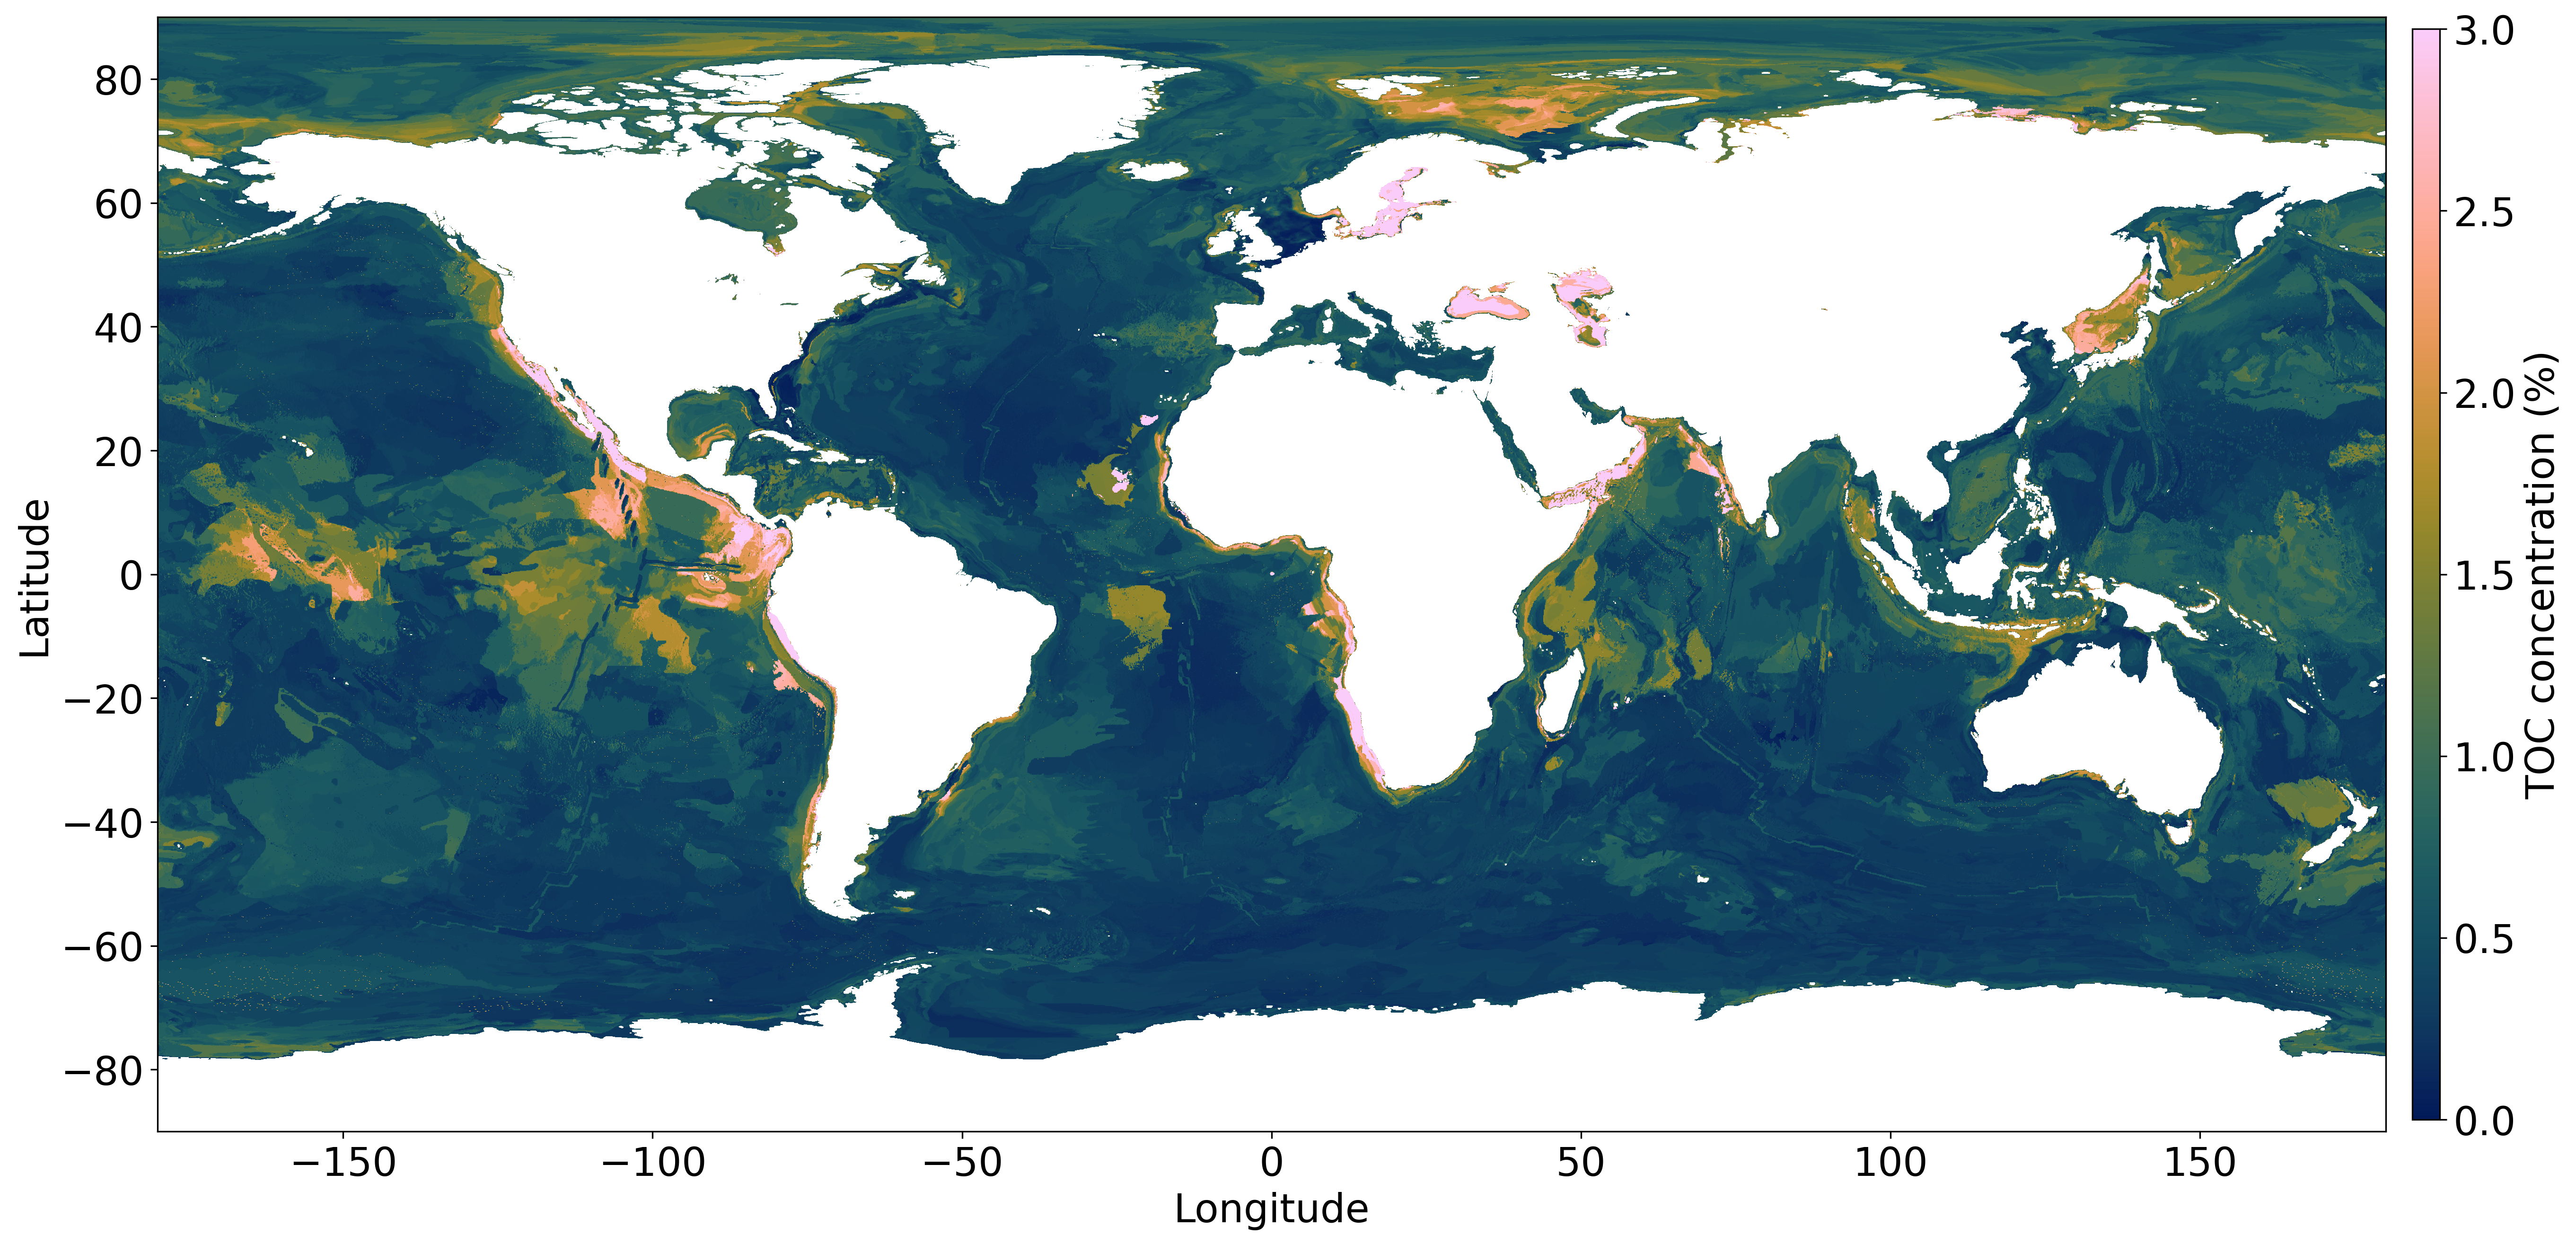
\includegraphics[width = 12 cm]{figures/f06.png}
    \caption{Global prediction map of TOC concentrations using a K-Nearest Neigbours algorithm with 5 nearest neighbors in the continental shelves and 4 nearest neighbors in the deep sea. The total TOC stock from the random forests model is 164.27 $Pg$ and the mean TOC concentration is 0.63\% for the entire ocean.}
    \label{fig:tocPercent_kNN}
\end{figure}

\begin{figure}[!htb]
    \centering
    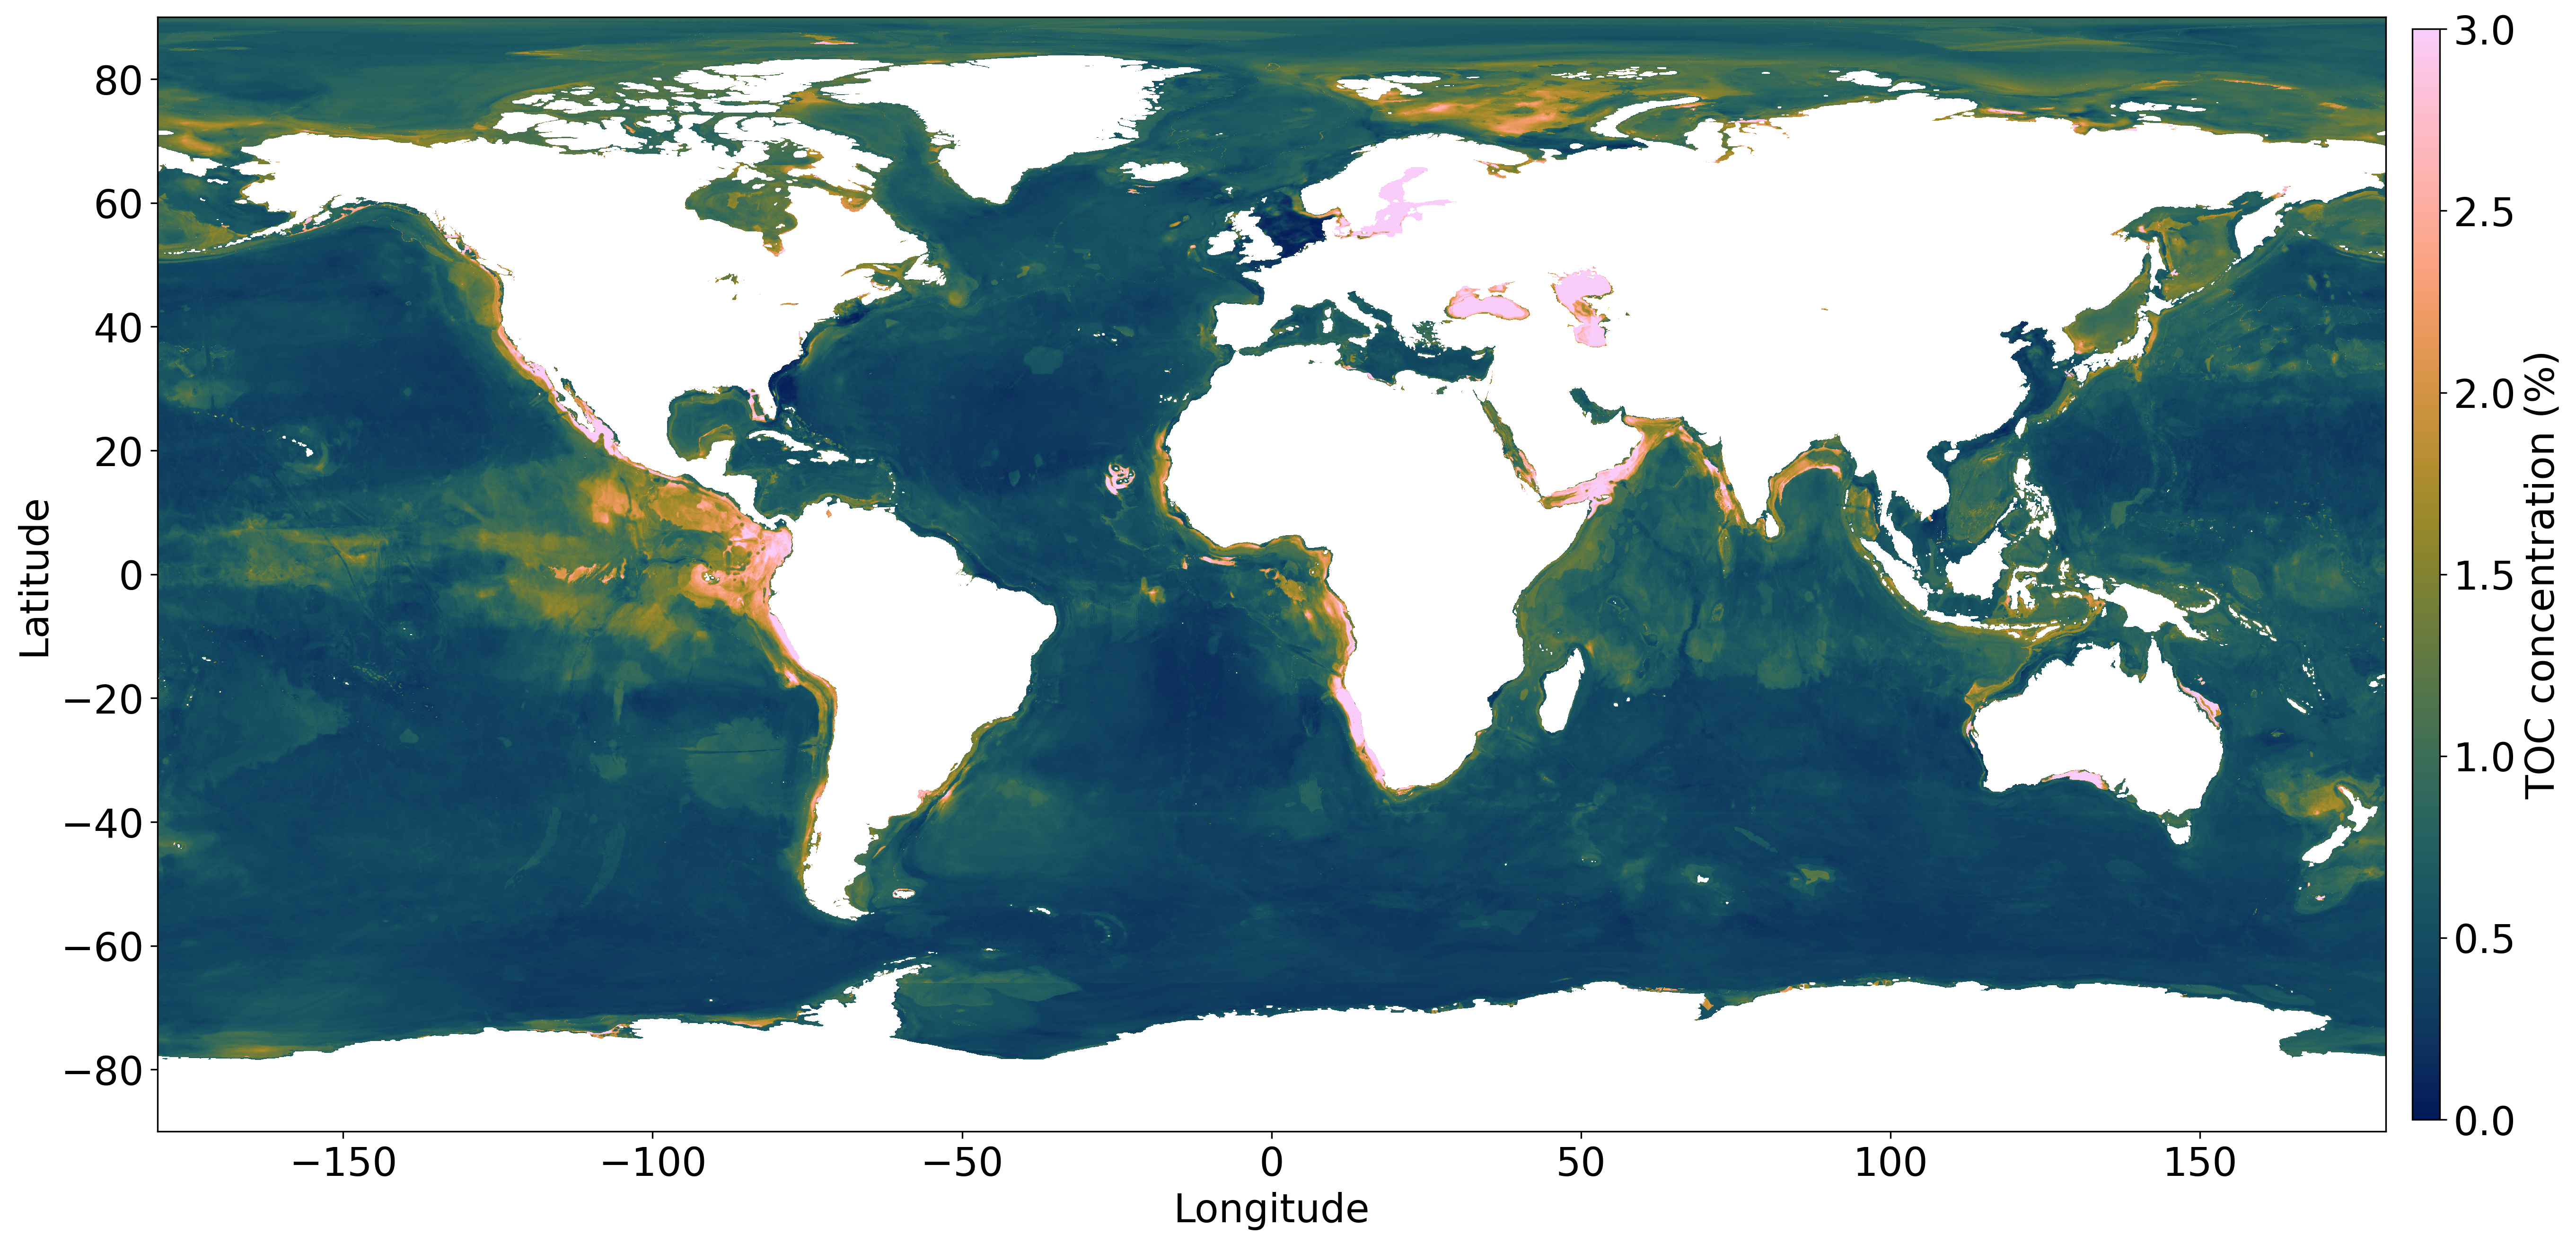
\includegraphics[width = 12 cm]{figures/f07.png}
    \caption{Global prediction map of TOC concentrations using a random forest algorithm with 100 estimators. The total TOC stock from the random forests model is 155.14 $Pg$ and the mean TOC concentration is 0.60\% for the entire ocean.}
    \label{fig:tocPercent_RF}
\end{figure}


\section{Information gain}
\label{appendix:informationgain}
In this paper, KL divergence, also known as information gain or relative entropy, has been used to quantify model uncertainty. As \cite{renyi1961measures} points out, the amount of information can be taken numerically equal to the amount of uncertainty concerning the model prediction. The mathematical derivation of KL divergence under the theoretical background of information theory \citep{shannoninformationgain1948} is presented below. The information entropy of a random variable $X$, with a probability distribution $P$ is represented as: 
\begin{equation}
\label{eq:entropy}
    H(P) = -\sum_i P(x_i) \log P(x_i)
\end{equation}

\cite{shannoninformationgain1948}'s definition of entropy determines the minimum channel capacity required to reliably transmit the information as encoded binary digits. Usually, the true distribution $P(X)$ denotes observed data, measurements, or an exact probability distribution. Here, $P(X)$ is constructed using a normal distribution with a mean value equal to Monte Carlo dropout prediction, and a standard deviation of 0.05 TOC\%, which arises from both technical handling and the precision of the weighing tool \citep{pape2020}. The predicted distribution $Q(X)$ is derived from the Monte Carlo dropout prediction ensemble. The measure $Q(X)$ typically represents a theoretical framework, a model, a description, or an approximation of $P(X)$. The cross entropy between $P(X)$ and $Q(X)$ measures the average number of binary digits to represent an event from $P(X)$, by $Q(X)$. It is represented as:

\begin{equation}
\label{eq:crossentropy}
    H(P, Q) = -\sum_i P(x_i) \log Q(x_i)
\end{equation}


The relative entropy, or the information gain measure the difference between the equations \ref{eq:crossentropy} and \ref{eq:entropy}, is represented as $D_{\text{KL}}(P \| Q)$,  or the information gain for a specific event \(x_i\) measures the cost in bits in modelling $P(x)$ with $Q(x)$. 

\begin{equation}
    D_{\text{KL}}(P \| Q) = H(P, Q) - H(P) = \sum_i P(x_i) \log\left(\frac{P(x_i)}{Q(x_i)}\right)
\end{equation}


$D_{\text{KL}}(P \| Q)$ is always non negative, remains well-defined for continuous distributions. To obtain the continuous distribution for the predicted distribution $Q(X)$, the prediction ensemble is binned into histograms, to obtain an approximate probability density function (PDF). This PDF is then modeled using curve fitting techniques, typically fitted to a Gaussian distribution (Algorithm \ref{alg:informationgain}). $D_{\text{KL}}(P \| Q)$, is calculated globally for each prediction, and plotted in the information gain map. 



\newpage
\section{Feature list}

File names adhere to the naming conventions discussed below. The naming structure is partitioned by underscores and periods in the following order: interface to which the gridded values refer to, quantity of values contained within the grid, units and reference values/units (e.g. meters below sea level), data source, statistic calculated (if applicable), grid pitch, and file extension.


SS – Sea surface – atmosphere interface (may also be average of the entire water column);

SF – Seafloor – water interface (may also be denoted by GL);

GL   – Ground level (e.g. bottom of pure liquid, top of dirt);

(r50 km) - Raw feature and feature averaged at a 50km radius used.

Units referenced are as follows:

KGM3 - kilogram per cubic meter;
MS - meters per second;
KM - kilometer;
M\_ASL - meters above sea level (i.e. meters referenced to sea level);
MWM2 - milliwatt per square meter;
TGCYR - terragram of carbon per year;
TGYR - terragram per year;
MA - megaannum;
M - meters;
MGCM2 - milligram of carbon per square meter;
DEG - degree;
S - seconds.

Most of the features presented below have been collected by  \cite{lee_2020_3675364} and \cite{benjamin_j_phrampus_2019_3459805}. The new datasets including the additions from this work are uploaded in (zenodo link).


\begin{longtable}{|p{0.4\textwidth}|p{0.35\textwidth}|p{0.25\textwidth}|}
    \hline
      \textbf{Feature} & \textbf{Explanation} & \textbf{Data Source} \\
      \hline
      \endfirsthead
      \hline
      \textbf{Feature name} & \textbf{Explanation} & \textbf{Data Source} \\
      \hline
      \endhead
        GL \_COAST \_FROM \_LAND \_IS \_1.0 \_ETOPO2v2.5m.nc (raw, r50km) & Coastline, with a binary indicator for the presence of coastline. This dataset is derived from ETOPO2v2, a 2-minute gridded global relief data for land boundary  &  \cite{ETOPO2v22006}\\
        \hline 
        GL \_COAST \_FROM \_SEA \_IS \_1.0 \_ETOPO2v2.r50km.men.5m.nc (raw, r50km) & Coastline with a binary indicator for the presence of coastline using ETOPO2v2 relief data for ocean boundary & \cite{ETOPO2v22006} \\
        \hline 
        GL \_DIST \_TO \_COAST \_KM \_ETOPO.r50km.men.5m.grd (raw, r50km)&  Distance from ocean grid points to the nearest coast. & \cite{ETOPO2v22006} \\
        \hline 
        GL \_ELEVATION \_M \_ASL \_ETOPO2v2.r50km.men.5m.grd (raw, r50km)&  Elevation data from ETOPO2v2, representing heights above sea level & \cite{ETOPO2v22006} \\
        \hline 
        GL \_RIVERMOUTH \_CO2 \_TGCYR-1 \_ORNL.r50km.men.5m.grd (raw, r50km)& Carbon dioxide flux at river mouths, measured in teragrams of carbon per year (Tg C/yr) &  \cite{ONRL2011}\\
        \hline 
        GL \_RIVERMOUTH \_DOC \_TGCYR-1 \_ORNL.r50km.men.5m.grd (raw, r50km)& Dissolved organic carbon flux at river mouths (Tg C/yr) & \cite{ONRL2011} \\
        \hline 
        GL \_RIVERMOUTH \_HCO3 \_TGCYR-1 \_ORNL.r50km.men.5m.grd (raw, r50km)& bicarbonate \ce{HCO3-} flux at river mouths (Tg C/yr) & \cite{ONRL2011} \\
        \hline 
        GL \_RIVERMOUTH \_POC \_TGCYR-1 \_ORNL.r50km.men.5m.grd (raw, r50km)& Particulate organic carbon flux at river mouths (Tg C/yr) &  \cite{ONRL2011}\\
        \hline 
        GL \_RIVERMOUTH \_TSS \_TGYR-1 \_ORNL.r50km.men.5m.grd (raw, r50km) & Total suspended solids flux at river mouths (50 km resolution) (Tg C/yr) & \cite{ONRL2011} \\
        \hline 
        %\newpage
        GL \_TOT \_SED \_THICK \_M \_CRUST1 \_NOAA.r50km.men.5m.grd (raw, r50km) & Total sediment thickness in the earth's crust in $m$  & \cite{CRUST1_NOAA2013} \\
        \hline 2N2 \_ocean \_eot20 \_modified.nc;K1 \_ocean \_eot20 \_modified.nc;K2 \_load \_eot20 \_modified.nc;K2 \_ocean \_eot20 \_modified.nc;M2 \_load \_eot20 \_modified.nc;M2 \_ocean \_eot20 \_modified.nc;M4 \_load \_eot20 \_modified.nc;M4 \_ocean \_eot20 \_modified.nc;MF \_load \_eot20 \_modified.nc;MF \_ocean \_eot20 \_modified.nc;MM \_load \_eot20 \_modified.nc;MM \_ocean \_eot20 \_modified.nc;N2 \_load \_eot20 \_modified.nc;N2 \_ocean \_eot20 \_modified.nc;O1 \_load \_eot20 \_modified.nc;O1 \_ocean \_eot20 \_modified.nc;P1 \_load \_eot20 \_modified.nc;P1 \_ocean \_eot20 \_modified.nc;Q1 \_load \_eot20 \_modified.nc;S1 \_load \_eot20 \_modified.nc;S1 \_ocean \_eot20 \_modified.nc;S2 \_load \_eot20 \_modified.nc;S2 \_ocean \_eot20 \_modified.nc;SA \_load \_eot20 \_modified.nc;SA \_ocean \_eot20 \_modified.nc; SSA\_load\_eot20\_modified.nc; SSA\_ocean\_eot20\_modified.nc & \cite{HartDavis2021EOT20} provides global atlases of both ocean and load tides are provided, containing information about the amplitudes and phases of seventeen tidal constituents(ocean and load) for the global ocean. These constituents include: 2N2, J1, K1, K2, M2, M4, MF, MM, N2, O1, P1, Q1, S1, S2, SA, SSA, and T2, that extends across the entire global ocean ranging from 66°S to 66°N. For higher latitudes, the FES2014b model is used to fill in the gaps. Eleven satellite altimetry missions contribute to this model. & \cite{HartDavis2021EOT20} \\
        \hline 
        ChlorSummerMean.nc & Average chlorophyll-alpha concentration during summer &  \cite{nasaaqua}\\
        \hline 
        ChlorWinterMean.nc & Average chlorophyll-alpha concentration during winter &  \cite{nasaaqua}\\
        \hline 
        DERIVATIVE \_GL \_ELEVATION \_M \_ASL \_ETOPO2v2.5.nc & Gradient of elevation from ETOPO2v2.5 data &  \\
        \hline 
        GL \_HEATFLUX \_MWM2 \_Becker.5m.nc & Oceanic heat flux data(exchange of heat energy between the ocean surface and the atmosphere) in megawatts per square meter($MW/m^2$) & \cite{becker2014} \\
        \hline
        GL \_LAND \_IS \_1.0 \_ETOPO2v2.5m.nc & Land mask data & \cite{ETOPO2v22006} \\
        \hline 
        POROSITY \_global \_prediction.grd & Global prediction map for porosity of surface sediments using a random forest method  & \cite{Martin2005Porosity} \\
        \hline 
        SF \_ACTIVE \_SEAMOUNTS \_KIM.r10km.wct.5m.grd & Active(volcanically) seamounts location data at a 10 km resolution & \cite{KIM2011} \\
        \hline 
        SF \_AVG \_SEA \_DENSITY \_KGM3 \_DECADAL \_MEAN \_woa13x.5m.grd (raw, r50km)& Mean sea density in $kg/m^3$ over a decade &  \cite{WOA13X2013}\\
        \hline 
        SF \_COASTLINE \_IS \_1.0.5m.nc & Coastline data &  \cite{lee_2020_3675364}\\
        \hline 
        SF \_CURRENT \_EAST \_MS \_2012 \_12 \_HYCOMx.5m.grd;SF \_CURRENT \_NORTH \_MS \_2012 \_12 \_HYCOMx.5m.grd;SF \_CURRENT \_MAG \_MS \_2012 \_12 \_HYCOMx.5m.grd (raw, r50km)& Ocean bottom current data for the east-west, north-south component and total magnitude using the HYCOM model in December 2012 in $m/s$ & \cite{HYCOM2014} \\
        \hline  
        SF \_GRAINSIZE \_D16 \_MM \_NGDC.5m.nc;SF \_GRAINSIZE \_D50 \_MM \_NGDC.5m.nc;SF \_GRAINSIZE \_D84 \_MM \_NGDC.5m.nc & Grainsize data with the 16th percentile (D16), median (D50) and the 84th percentile (D84) & \cite{ngdc1976} \\
        \hline 
        SF \_SEA \_BULKMODULUS \_MPA \_DECADAL \_MEAN \_woa13x.5m.nc & Sea bulk modulus in mega pascals(MPa) averaged over a decade & \cite{WOA13X2013} \\
        \hline 
        SF \_SEA \_CONDUCTIVITY \_SM \_DECADAL \_MEAN \_woa13v2x.5m.grd(raw, r50km)  & Average conductivity of seawater(dissolved ions) at the sea surface over a decade in siemens per meter($S/m$) & \cite{WOA13X2013} \\
        \hline 
        SF \_SEA \_OXYGEN \_MLL \_DECADAL \_MEAN \_woa13v2x.5m.grd(raw, r50km) & Average dissolved sea oxygen in millilitre per litre over a decadal mean & \cite{WOA13X2013} \\
        \hline 

        SF \_SEA \_OXYGEN \_PCTSAT \_DECADAL \_MEAN \_woa13v2x.5m.grd(raw, r50km) & Sea oxygen percentage saturation averaged over a decade & \cite{WOA13X2013}\\
        \hline 
        SF \_SEA \_PRESSURE \_MPA \_DECADAL \_MEAN \_woa13x.5m.nc & Sea pressure in mega pascals($MPa$) averaged over a decade. & \cite{WOA13X2013} \\
        \hline 
        SF \_SEA \_SALINITY \_PSU \_DECADAL \_MEAN \_woa13v2x.5m.nc & Sea salinity in practical salinity units averaged over a decade & \cite{WOA13X2013} \\
        \hline 
        SF \_SEA \_SEA \_OXYGEN \_UTILIZATION \_MOLM3 \_DECADAL \_MEAN \_woa13v2x.5m.grd(raw, r50km) & Sea oxygen utilization in mol/m³ averaged over a decade &  \cite{WOA13X2013}\\
        \hline 
        SF \_SEA \_TEMPERATURE \_C \_DECADAL \_MEAN \_woa13v2x.5m.grd(raw, r50km) &  Sea Temperature in Celcius averaged over a decade & \cite{WOA13X2013} \\
        \hline 
        SL \_GEOID \_M \_ABOVE \_WGS84 \_NGA \_egm2008.5m.grd & Height of the geoid above the WGS84 reference ellipsoid, in meters($m$), and referenced to the National Geospatial-Intelligence Agency (NGA)
& \cite{NGA_EGM20082008} \\
        \hline 
        SS \_BIOMASS \_BACTERIA \_LOG10 \_MGCM2 \_WEI2010x.5m.grd(raw, r50km); SS \_BIOMASS \_FISH \_LOG10 \_MGCM2 \_WEI2010x.5m.grd(raw, r50km); SS \_BIOMASS \_INVERTEBRATE \_LOG10 \_MGCM2 \_WEI2010x.5m.grd(raw, r50km); SS \_BIOMASS \_MACROFAUNA \_LOG10 \_MGCM2 \_WEI2010x.5m.grd(raw, r50km); SS \_BIOMASS \_MEGAFAUNA \_LOG10 \_MGCM2 \_WEI2010x.5m.grd(raw, r50km); SS \_BIOMASS \_MEIOFAUNA \_LOG10 \_MGCM2 \_WEI2010x.5m.grd(raw, r50km); SS \_BIOMASS \_TOTAL \_LOG10 \_MGCM2 \_WEI2010x.5m.grd(raw, r50km); & Distribution of mean biomass predictions for (a)bacteria, (b)fishes, (c)invertebrates, (d)macrofauna, (e)megafauna, and (f)meiofauna. The mean biomass was computed using random forest algorithm. The total biomass was combined from predictions of bacteria, meiofauna, macrofauna, and megafauna biomass. Predictions were smoothed by Inverse Distance Weighting interpolation to 0.1 degree resolution and displayed in logarithm scale (base of 10), which is then converted to 5 arc minute grids by \cite{LeeTOCkNN} & \cite{WEI2010} \\
        \hline 
        SS \_CHLOROPHYLL \_LOG \_MG \_M3 \_MODIS \_Aqua \_MISSION \_MEANx.5m.grd(raw, r50km); SS \_PIC \_LOG \_MOL \_M3-1 \_MODIS \_Aqua \_MISSION \_MEANx.5m.grd(raw, r50km); SS \_POC \_LOG \_MOL \_M3-1 \_MODIS \_Aqua \_MISSION \_MEANx.5m.grd(raw, r50km)  & The Moderate Resolution Imaging Spectroradiometer (MODIS), is a 36-band spectroradiometer measuring visible and infrared radiation and obtaining data that are being used to derive the near-surface concentration of chlorophyll-a (chlor\_a) in $mg m^-3$. It is calculated using an empirical relationship derived from in situ measurements of chlor\_a, concentrations of Particulate Organic Carbon(POC) and Particulate Inorganic Carbon(PIC) (i.e., calcium carbonate or calcite) and blue-to-green band ratios of in situ remote sensing reflectances (Rrs). & \cite{nasaaqua} \\
        \hline 
        SS \_CORIOLIS.5m.nc  & Coriolis data, generated using empirical means & \cite{lee_2020_3675364}\\
        \hline 
        SS \_DENSITY \_KGM-3 \_SACD \_Aquarius \_MISSION \_MEANx.5m.grd & The Aquarius/SAC-D satellite mission, launched on 10 June 2011, was a joint venture between NASA and the Argentinean Space Agency (CONAE). The mission featured the sea surface salinity sensor Aquarius and was the first mission with the primary goal of measuring sea surface salinity (SSS) from space. The monthly maps of sea surface density are derived from Aquarius sea surface salinity and ancillary sea surface temperature.  & \cite{nasaaquarius} \\
        \hline 

         SS \_GEOID \_ANOMALY \_NGA \_egm2008.5m.nc(raw, r50km) & The regional Free-air and Bouguer gravity anomaly grids (averaged over 2,5 arc-minute by 2,5 arc-minute) are computed at BGI from the EGM2008 spherical harmonic coefficients & \cite{NGA_EGM20082008} \\
        \hline 
        SS \_MIXED \_LAYER \_DEPTH \_MAX \_M \_Goyetx.5m.grd(raw, r50km); 
         SS \_MIXED \_LAYER \_DEPTH \_MIN \_M \_Goyetx.5m.grd(raw, r50km)& shows the geographical distribution of the maximum and minimum depth($m$) of the mixed layer & \cite{goyetMLD} \\
        \hline
        SS \_PHOTO \_AVAIL \_RAD \_EINSTEIN \_M-2 \_DAY \_SNPP \_VIIRS \_MISSION \_MEANx.5m.grd(raw, r50km); SS \_PHYTO \_ABSORPTION \_443NM \_M-1 \_SNPP \_VIIRS \_MISSION \_MEANx.5m.grd  & Daily average photosynthetically available radiation (PAR) at the ocean surface in $Einstein/m^2/day$ The Visible Infrared Imaging Radiometer Suite (VIIRS) on the Suomi National Polar-orbiting Partnership (SNPP) have been developed for global ocean color products. PAR is defined as the quantum energy flux from the Sun in the 400-700nm range. For ocean color applications, PAR is a common input used in modeling marine primary productivity. An average of the sensors and the 443 $nm$ wavelength maps are used as features& \cite{nasaaqua}\\
        \hline
         SS \_WAVE \_DIRECTION \_DEG \_2012 \_12 \_WAVEWATCH3x.5m.grd(raw, r50km); SS \_WAVE \_HEIGHT \_M \_2012 \_12 \_WAVEWATCH3x.5m.grd(raw, r50km); SS \_WAVE \_PERIOD \_S \_2012 \_12 \_WAVEWATCH3x.5m.grd(raw, r50km) & Mean Wave direction in $\°$, wave height in $m$ and wave period in $s$. Features are based on the 3rd generation wave model WAVEWATCH III®. & \cite{HYCOM2014} \\
        \hline 
        SS \_WINDSPEED \_MS-1 \_SACD \_Aquarius \_MISSION \_MEANx.5m.grd(raw, r50km) & Mean wind speed in $m/s$ fromtThe Aquarius/SAC-D satellite mission & \cite{nasaaquarius} \\
        \hline 
        TOU \_Jorgenson2022.nc & Global map of the total oxygen uptake (TOU) of the seabed. & \cite{TOU_JORGENSEN2022} \\
        \hline 
        litho\_maps\_type1\_.nc & Lithology map: Mudflats binary map (<0.05 $mm$) & \cite{garlan2018}  \\
        \hline 
        litho\_maps\_type2\_.nc & Lithology map: Fine sand binary map (0.05 $mm$ - 0.5 $mm$) & \cite{garlan2018} \\
        \hline 
        litho\_maps\_type3\_.nc & Lithology map: Sand binary map (0.5 $mm$ - 2 $mm$) & \cite{garlan2018} \\
        \hline 
        litho\_maps\_type4\_.nc & Lithology map: Clay binary map (<0.01 $mm$) & \cite{garlan2018}
        \hline 
        litho\_maps\_type5\_.nc & Lithology map: Gravel and stone binary map (>2 $mm$) & \cite{garlan2018}
        \hline 
        litho\_maps\_type6\_.nc & Lithology map: Bed rock binary map & \cite{garlan2018}
        \hline 
        lithology \_grain \_size \_global \_8.nc & Grain size distribution of sediments & \cite{garlan2018} \\
        \hline 
\caption{Feature list with description and references, that is used as input to all the models in the paper.}
\label{tab:myfirstlongtable}
\end{longtable}





\newpage
\section{Algorithms}
\begin{algorithm}
\caption{Neural Network Training with Batch Normalization and Dropout including Monte Carlo Dropout for inference}
\label{a2}
\begin{algorithmic}[1]
\REQUIRE Labeled dataset $D = \{(x_1, y_1), (x_2, y_2), ..., (x_N, y_N)\}$ \\
\hspace{13mm} $x_i$: feature vector for the $i$th label \\
\hspace{13mm} $y_i$: corresponding TOC\%
\STATE \textbf{Input:} feature vector $x_j$
\STATE \textbf{Output:} Predicted TOC\% $\text{predicted\%}$ for $x_j$
\STATE \textbf{Method:} Construct a neural network with 10 layers and 128 nodes per layer: $\phi(x, W, b)$
\STATE Apply batch normalization and dropout to each layer.
\STATE Initialize optimizer (e.g., Adam) with appropriate learning rate and parameters.
\STATE Initialize loss function (e.g., Mean Squared Error) for regression.
\STATE Train the neural network with $D$ for 1000 epochs:
\FOR{$\text{epoch} = 1$ \TO $\text{num\_epochs}$}
    \STATE Randomly shuffle the training dataset..
    \FOR{$(x_i, y_i)$ in $D$}
        \STATE Forward pass: compute predictions $\hat{y_i} = \phi(x_i, W, b)$.
        \STATE Compute target loss: $\text{loss}_{\text{target}} = \text{MSE}(y_i, \hat{y_i})$.
        \STATE Back-propagation: update weights and biases using optimizer, with $\text{loss}_{\text{target}}$ as the cost function.
    \ENDFOR
\ENDFOR
\STATE Set dropout to active during inference
\STATE Perform Monte Carlo dropout for $M$ forward runs:
\STATE \hspace{5mm} $\hat{y}^{\text{ensemble}}_j =  \phi(x_j, W, b, \text{dropout\_mask}_T)$
\STATE Predicted TOC\%, $\hat{y_j}$ for $x_j = \frac{1}{M}  \sum_{m=1}^{M} \hat{y}^{\text{ensemble}}_j$
\end{algorithmic}
\end{algorithm}


\begin{algorithm}
\caption{Calculating information gain for the predictions}
\label{alg:informationgain}
\begin{algorithmic}[1]
\REQUIRE Monte Carlo dropout prediction ensemble, $\hat{y}^{\text{ensemble}}$, for each grid cell
\FOR{each grid cell}
    \STATE Fit a gaussian probability density function $Q_j(x)$ for $\hat{y}^{\text{ensemble}}_j$ using histograms and curve fitting algorithm.
    \STATE Generate original distribution $P_j(x)$ with mean $\hat{y_j}$ and standard deviation 0.05 (sampling error).
    \STATE Calculate Kullback-Leibler divergence: \\
    \hspace{3mm} $D_{\text{KL}}(P_j \| Q_j) = \sum_i P_j(x_i) \log\left(\frac{P_j(x_i)}{Q_j(x_i)}\right)$
\ENDFOR
\end{algorithmic}
\end{algorithm}






\newpage
\section{Model interpretability using SHAP values}
Explaining and understanding why a model makes a certain prediction is as crucial as accuracy and uncertainty in the predictions. This becomes particularly challenging in high-dimensional spaces, where interpreting complex models can be more intricate compared to simpler yet less accurate models. \cite{lundberg2017shap} proposes a unified framework for interpreting predicitons, SHAP (SHapley Additive exPlanations). SHAP assigns importance values to each feature for a particular prediction, providing a comprehensive understanding of the model's decision-making process. In our supervised learning model $f$ trained on features $X \in \mathcal{X} \subseteq \mathbb{R}^d$ to predict outcomes $Y \in \mathcal{Y} \subseteq \mathbb{R}$, SHAP, a feature attribution method, considers the model predictions to be decomposed as a sum: $f(\mathbf{x}) = \phi_0 + \sum_{j=1}^{d} \phi(j, \mathbf{x})$, where $\phi_0$ is the baseline expectation (i.e., $\phi_0 = \mathbb{E}[f(\mathbf{x})]$) and $\phi(j, \mathbf{x})$ denotes the Shapley value of feature $j$ at point $x$. 


In our analysis, we aim to simplify the interpretation process by presenting the average importance of features across all predictions, from the deep sea and the continental shelves. All effects describe the behavior of the model and are not necessarily causal in the real world. 

\begin{figure}[!htb]
\includegraphics[width=12cm]{figures/f08.png}
\caption{Summary plot of Shapley values of the deep sea DNN model. The global porosity grid \citep{Martin2005Porosity} has the highest feature importance. Regions with high porosity lead to higher TOC concentrations, and vice versa. The biological features that includes biomass meiofauna \citep{WEI2010}, sea oxygen utilization \citep{WOA13X2013}, daily average PAR \citep{nasaaqua} show that higher biomass lead to higher TOC concentrations. On the other hand, higher oxygen saturation leads to oxic conditions, resulting in the oxidation of the organic carbon and hence lesser TOC concentration. The other features which dominate are the physical oceanographic features, where higher feature values result in lower TOC concentration, such as tidal features (Q1 loading, M2 constituent) \citep{HartDavis2021EOT20}, Sea bulk modulus \citep{WOA13X2013}, average sea conductivity \citep{WOA13X2013} and bottom current magnitude \citep{HYCOM2014} (strong bottom currents that inhibit sediment deposition).}
\label{fig:shap_do}
\end{figure}
\clearpagey

\begin{figure}[!htb]
\includegraphics[width=12cm]{figures/f09.png}
\caption{Summary plot of Shapley values of the continental shelf DNN model. The total oxygen uptake \citep{TOU_JORGENSEN2022} of the sea bed has the highest feature importance, with regions of higher oxygen uptake resulting in lower TOC concentrations, denoting oxic conditions. Regions with higher porosity \citep{Martin2005Porosity} result in higher TOC concentrations, while regions with lower porosity result in lower TOC concentration, but with lesser impact. The lithology map is a binary map. Regions with fine sand, with the grain size between 0.05 $mm$ and 0.5 $mm$(1, being the higher feature value) has low impact on the TOC concentration. Higher sediment thickness in the earth's crust lead to lower TOC concentration because of dilution \citep{Berner1982}. Higher sea surface POC and absorption of 443 $nm$ ocean color wave length results in higher TOC concentration, while lower values of the features do not impact the model output greatly. Physical oceanographic features such as higher wind speed and bottom currents result in lesser TOC concentration, due to higher resuspension of sediments.   It can be seen that the feature importance is not clearly defined as the deep ocean, because of the complex dynamics in continental shelves. Similar to the deep sea, the higher average seawater conductivity results in lower TOC concentration. }
\label{fig:shap_cs}
\end{figure}


The summary plot in Figures \ref{fig:shap_do} and \ref{fig:shap_cs} combines the feature importance with feature effects. The summary plot displays Shapley values representing the impact of features on predictions. Each point represents a Shapley value for a feature and an instance. The y-axis position indicates the feature, while the x-axis position corresponds to the Shapley value. Feature values are represented by color, ranging from low(blue) to high(red). To visualize feature importance, points are spread along the y-axis to reveal the distribution of Shapley values per feature. The features are ordered based on their importance, determined by the mean absolute Shapley values across all predictions. The Shapley value is expressed in the same units as the TOC concentration. This indicates the extent to which a specific feature value influences the TOC concentration, whether it drives it towards higher or lower values.

\newpage
\section{TOC stock in different marine regions}
The table in Table \ref{tab:TOCStockOcean} breaks down how much TOC stock is found in different parts of the ocean. Each region is listed, showing how much TOC is there. Here we show a visualisation of the different regions in Figure \ref{fig:TOCStockOceans}.

In Figure \ref{fig:TOCStockOceansWaffle}, we use a waffle chart to make it easier to see how the TOC is split among these regions. It's like dividing a pie into slices, but here we use squares. With a total of about 171 $Pg$ of TOC worldwide, the South Pacific Ocean gets the biggest share, while the Baltic Sea gets the smallest.
\begin{figure}[!htb]   
\centering
   \includegraphics[width = 12cm]{figures/f10.png}
   \caption{TOC stocks in different oceans}
   \label{fig:TOCStockOceans}
\end{figure}

\begin{figure}[!htb]
   \centering
   \includegraphics[width = 12cm]{figures/f11.png}
   \caption{TOC stocks in different oceans: Waffle chart}
   \label{fig:TOCStockOceansWaffle}
\end{figure}


\newpage
\authorcontribution{Burwicz-Galerne, Ewa did the data collection of the oceanographic features and TOC concentration labels. Wallmann, Klaus and Burwicz-Galerne, Ewa did the feature selection and provided inputs on the geoscientific part of the manuscript. Braack, Malte provided inputs on cleaning the data and building the models. Parameswaran, Naveenkumar and Gonzalez, Everardo developed the model code and performed the runs. Parameswaran, Naveenkumar prepared the manuscript with contributions from all co-authors.} 


\competinginterests{The authors declare that they have no conflict of interest.} %% this section is mandatory even if you declare that no competing interests are present

%\disclaimer{TEXT} %% optional section

\begin{acknowledgements}
This work was partially funded by the Cluster of Excellence `The Ocean Floor – Earth’s Uncharted Interface' (EXC 2077) financed by Deutsche Forschungsgemeinschaft (DFG) - Project number 390741603 hosted by the Research Faculty MARUM - Center for Marine Environmental Sciences, University of Bremen, Germany.

The first author wants to thank the Helmholtz School for Marine Data Science (MarDATA), for direct financial support. 

AI tools has been used to correct the manuscript, and optimize the code.
\end{acknowledgements}





\newpage
\bibliographystyle{copernicus}
\bibliography{ref.bib}


\end{document}
